% Not All Errors Are Equal: Consequence-Aware Reasoning Compute Allocation
% arXiv submission version

\documentclass{article}
\usepackage{times}
\usepackage[utf8]{inputenc}
\usepackage[T1]{fontenc}
\usepackage{natbib}
\input{math_commands.tex}

\usepackage[hidelinks,colorlinks=false]{hyperref}
\usepackage{url}
\usepackage{graphicx}
\usepackage{amsmath}
\usepackage{amssymb}
\usepackage{algorithm}
\usepackage{algorithmic}
\usepackage{booktabs}
\usepackage{multirow}
\usepackage{microtype}
\usepackage[margin=1.4in]{geometry}

\title{Not All Errors Are Equal:\\Consequence-Aware Reasoning Compute Allocation}

\author{
Jingbo Wen$^{1}$ \quad
Liang He$^{2,\ast}$ \quad
Ziqi He$^{1}$ \\[4pt]
$^{1}$The University of Sydney \\
$^{2}$Shanghai Institute of Optics and Fine Mechanics \\[4pt]
\texttt{hel@siom.ac.cn} \\[2pt]
$^\ast$Corresponding authors
}

\begin{document}

\maketitle

\begin{abstract}
Modern reasoning models can allocate different amounts of test-time computation, such as thinking tokens, model calls, or compute budget, to different tasks. Existing methods generally drive this allocation by predicted difficulty and spend more compute where it is expected to raise accuracy. This implicitly assumes that all failures cost the same, since an accuracy objective weights every task equally. However, such an assumption does not hold in deployment: A typo in a log message and a migration that corrupts a production database both count as one benchmark failure, but their real-world costs are fundamentally different. To fill this gap,
we propose consequence-aware test-time compute allocation. Instead of routing compute only by predicted difficulty, we use a lightweight predictor to estimate from the issue text how costly a task would be if solved incorrectly. The scheduler then routes higher-consequence tasks to larger compute tiers or higher thinking budgets under the same total budget. We conduct main experiments on SWE-bench Lite, evaluate cross-dataset behavior on Multi-SWE-bench mini, replicate the full allocation comparison on a disjoint database/ORM pool from SWE-bench Verified, and run an end-to-end out-of-domain probe on BIRD text-to-SQL, covering
990 tasks in total. Our results reveal that consequence and difficulty are approximately orthogonal under various annotations, and that current thinking models do not allocate compute sufficiently according to consequence. Moreover, our issue-only predictor never misclassifies a high-consequence task as low-consequence on any of the four task pools ($0/97$). 
Under matched compute budgets --- in a simulation over cached outcomes of $16$ public SWE-bench systems spanning capability tiers --- the fully deployment-time consequence-only scheduler reduces cost-weighted loss by $21.8\%$ ($17.7$--$29.9\%$ across cost mappings) relative to difficulty-aware routing and retains $93.6\%$ of the corresponding oracle gain; the pattern persists when a single fixed model allocates real best-of-$k$ attempts. A priority-aware variant that additionally uses empirical marginal-gain information further reduces loss by $30.7\%$, showing the potential value of estimating where extra compute changes the outcome.
Notably, difficulty-aware routing with outcome-derived difficulty performs worse than random --- many of the hardest tasks remain unsolved even at the premium tier --- while deployment-time predicted difficulty merely matches random; under every variant, difficulty routing trails consequence routing.
\end{abstract}

\section{Introduction}
\label{sec:intro}

Modern reasoning models, such as OpenAI's o-series, DeepSeek-R1,
Anthropic's Claude with extended thinking, and Qwen3-Thinking, can decide
how much test-time computation to spend on each input~\citep{li2025reasoningllms,liu2025efficientreasoning}. In practice, they
vary how long they think from task to task, often producing longer
reasoning traces on inputs that appear more difficult~\citep{alomrani2025reasoningbudget,zhu2025adaptivethinking,pan2025slowthinking}. The same principle
is pursued explicitly in adaptive test-time compute, where learned
routers~\citep{damani2024learning}, compute-difficulty scaling
laws~\citep{snell2024scaling}, self-assessment-driven early
stopping~\citep{manvi2024adaptive}, and budgeted verifier-call
scheduling~\citep{qu2026adaptivetesttime} differ in mechanism but follow a common
rule, namely that harder tasks deserve more compute.


This principle is natural for benchmarks that optimize average accuracy under a compute budget. In such settings, each task contributes one unit to the final score, and every failure is assumed to be interchangeable~\citep{alomrani2025reasoningbudget}. However, this is not how deployment works, and such an assumption generally does not hold in deployment. Consider two failures a coding assistant might produce on the same day: a typo in a log message and a database migration that silently corrupts a production table under a race condition. A benchmark records both as one failed task, but in deployment their costs are nowhere near equal: preventing the migration error is worth far more compute, even when the two are equally hard to fix.

This deployment mismatch exposes a missing term in current LLM adaptive-compute objectives. The closest prior framing is rational metareasoning~\citep{russell1991right, hay2012selecting,
yang2024rational}, which treats computation as an action whose value
depends on its expected utility. From this perspective, additional reasoning is useful only when the expected reduction in downstream loss exceeds the cost of computation~\citep{alomrani2025reasoningbudget}. Modern LLM implementations of adaptive compute, however, typically collapse this utility term into a uniform accuracy objective~\citep{li2025reasoningllms}. We therefore move beyond difficulty-aware allocation and cast consequence-aware allocation as a cost-weighted problem: for each task, a scheduler should choose a compute tier that trades off the price of additional computation against the expected consequence-weighted error. When all tasks have equal error cost, this objective reduces to standard accuracy maximization under a compute budget~\citep{alomrani2025reasoningbudget}. When error costs vary, however, difficulty alone is no longer a sufficient routing signal.

\begin{figure}[t]
\centering
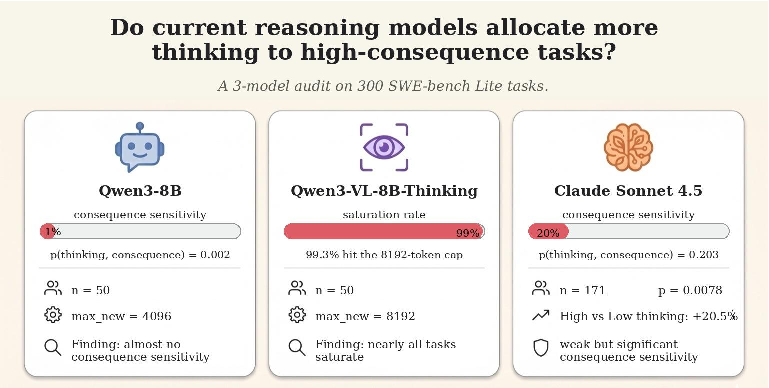
\includegraphics[width=\linewidth]{fig_motivation.pdf}
\caption{\textbf{Three contemporary thinking models do not sufficiently
allocate compute by consequence.} Each panel summarizes one model's
relationship between actual thinking length and our consequence label
on SWE-bench Lite tasks. Qwen3-8B's thinking length is uncorrelated
with consequence ($\rho = 0.002$). Qwen3-VL-8B-Thinking pins
$99.3\%$ of tasks at its 8192-token cap. Claude Sonnet 4.5 with
extended thinking shows a statistically significant but weak
consequence sensitivity ($\rho = 0.20$, $p = 0.008$, $n = 171$).
Across three different allocation mechanisms, none exhibits sufficient
consequence sensitivity to explain the gains of consequence-aware
routing observed later in the paper.}
\label{fig:motivation}
\end{figure}

One might hope that sufficiently strong reasoning models already learn
this distinction implicitly. If high-consequence tasks naturally induce
longer reasoning traces, then an explicit cost signal would be unnecessary. We test this possibility directly by
auditing contemporary thinking models on SWE-bench Lite (three of
which are shown in Figure~\ref{fig:motivation}). The results show three different failure
modes. Qwen3-8B varies its thinking length, but that variation is
essentially uncorrelated with consequence
($\rho = 0.002$). Qwen3-VL-8B-Thinking reaches its 8192-token cap on
$99.3\%$ of tasks, leaving almost no room for task-specific allocation.
Claude Sonnet 4.5 with extended thinking shows a statistically
significant relationship between thinking length and consequence
($\rho = 0.20$, $p = 0.008$, $n = 171$), but the effect is small:
high-consequence tasks receive only $20.5\%$ more thinking than
low-consequence tasks. The same pattern holds for OpenAI's o4-mini on
the identical task sample ($\rho = 0.24$, $+31.4\%$ reasoning tokens
for high- vs low-consequence tasks), while DeepSeek-R1 saturates even
a $24{,}000$-token reasoning budget on $54\%$ of the same tasks, with
no significant consequence signal in which tasks saturate
(\S\ref{sec:audit}).
Thus, existing thinking models exhibit either no
consequence signal, saturation, or only weak consequence sensitivity.

Motivated by this gap, we propose consequence-aware test-time
compute allocation.
The method separates two decisions that are often conflated ---
existing cost-aware routing prices the \emph{compute} side of the
trade-off~\citep{shirkavand2025costaware}, while the cost of
\emph{errors} is left uniform.
First, a lightweight predictor estimates the deployment-time
cost of an error directly from the issue text, before the task is
solved.
Second, a scheduler uses this predicted consequence to route
higher-consequence tasks to larger compute tiers, or equivalently to
larger thinking budgets, under the same total compute budget as a
difficulty-based baseline.
The reasoning model itself is not retrained;
the intervention operates entirely at the scheduling layer.

The remainder of the paper builds the empirical case in four steps.

\begin{itemize}
\item[(1)] \textbf{Consequence is not difficulty, nor a disguised
confidence signal.} On $300$ SWE-bench Lite tasks, consequence
remains nearly orthogonal to difficulty across rule-based,
LLM-with-patch, issue-only, and human-majority labels. Moreover, after controlling for both
difficulty and cross-model pass-rate variance, consequence still
explains an additional $26.4$ percentage points of cost-weighted
marginal value ($+55.7\%$ relative; \S\ref{sec:cons},
\S\ref{sec:whyfail}).

\item[(2)] \textbf{Existing thinking models are not sufficiently
consequence-aware.} The audit in \S\ref{sec:audit} (with three of the
mechanisms shown in Figure~\ref{fig:motivation}) reveals
distinct allocation failure patterns: no consequence signal in
Qwen3-8B, near-universal saturation in Qwen3-VL-8B-Thinking, majority
saturation in DeepSeek-R1 even at a $24{,}000$-token budget, and weak
but insufficient consequence sensitivity in both Claude Sonnet 4.5 and
o4-mini (\S\ref{sec:audit}).

\item[(3)] \textbf{Consequence can be predicted before solving.} A
Qwen2.5-7B-Instruct~\citep{qwen2025qwen25} issue-only predictor, which sees only the issue text and file
path, agrees with the Qwen2.5-7B-Instruct with-patch reference at Cohen's
$\kappa = 0.572$~\citep{cohen1960kappa}. A cross-model Claude issue-only predictor reaches
$\kappa = 0.379$. Crucially, neither predictor ever misclassifies a
high-consequence task as low-consequence --- across the $300$
SWE-bench Lite tasks for both predictors, and across all $399$
judge-labeled Multi-SWE-bench mini tasks for the Qwen predictor
(\S\ref{sec:pred}, Appendix~\ref{app:crossdataset}). This avoids
the most dangerous under-allocation error on all $700$ tasks we
study.

\item[(4)] \textbf{Deployment-time consequence routing improves
cost-weighted allocation, and marginal-gain information improves it
further.} Under matched compute on a $16$-model SWE-bench compute-tier
benchmark, the Qwen issue-only consequence predictor reduces
cost-weighted loss by $21.8\%$ relative to difficulty-aware routing and
retains $93.6\%$ of the consequence-oracle gain. A priority-aware
variant that additionally uses empirical marginal-gain information
reduces loss by $30.7\%$, showing the further value of estimating where
extra compute changes the outcome. The same analysis also explains why
difficulty-aware routing can underperform random: the hardest tasks
often have the lowest marginal gain from extra compute, because they
remain unsolved at every available tier (\S\ref{sec:exp},
\S\ref{sec:whyfail}).
\end{itemize}

\section{Related Work}

\textbf{Adaptive test-time compute.}
A growing body of work studies how much computation a language model
should spend on each input. \citet{snell2024scaling} analyze the effectiveness of different test-time scaling strategies and derive difficulty-dependent compute-optimal policies for using a fixed inference budget. \citet{damani2024learning}
train a reward predictor to allocate compute according to expected
accuracy gain. \citet{manvi2024adaptive} train models to predict mid-generation
whether further compute would improve the answer, enabling early
stopping. Although
these methods differ in implementation, they share the same underlying
objective: spend compute where it is expected to improve average
accuracy. Our work asks a complementary question. When two tasks have
similar expected accuracy gains but very different costs of failure,
an accuracy-driven router treats them as equivalent, whereas a
deployment-oriented scheduler should not. We therefore keep the
reasoning model unchanged and change the routing signal from predicted
difficulty or confidence to predicted consequence.

\textbf{Rational metareasoning.}
The decision-theoretic view of computation as a costly action dates
back to rational metareasoning~\citep{russell1991right,
hay2012selecting}. In this framework, additional computation is useful
only when its expected utility exceeds its computational cost.
This perspective is closely aligned with our formulation: Whether a task is worth more compute depends not only on how much that compute would improve the answer, but on how costly an error would be. Recent work
has begun to apply rational metareasoning to large language
models~\citep{yang2024rational}. However, in most LLM adaptive-compute
settings, utility is operationalized as accuracy, reward, or confidence
rather than as a task-dependent cost of error.

\textbf{Cost-sensitive learning and selective prediction.}
Cost-sensitive learning studies classification under asymmetric error
costs~\citep{elkan2001foundations}, while selective prediction allows
a model to abstain when it is uncertain~\citep{geifman2017selective}.
Both lines of work recognize that errors are not interchangeable. The
difference lies in where the cost signal is used. Cost-sensitive learning
typically changes the training objective or decision rule, and selective prediction decides whether to answer at all. In contrast, we use the cost signal at compute time: the model still answers every
task, but the scheduler decides how much computation the task should receive before answering. This makes the approach compatible with existing reasoning models without retraining.

\textbf{Software-engineering benchmarks.}
We use SWE-bench Lite~\citep{jimenez2023swebench} as our primary testbed and a 400-task subset of Multi-SWE-bench~\citep{ma2024multiswebench}
for cross-dataset validation. Software-engineering tasks are a natural setting for consequence-aware allocation because they contain both large variation in task difficulty and large variation in deployment
risk. A documentation typo, a parser edge case, a permission bug, and a database migration error may all appear as single pass/fail tasks in a benchmark, yet their real-world consequences differ substantially.
The availability of issue reports, file paths, and gold patches also allows us to compare deployment-time issue-only prediction with with-patch consequence labels.

\section{Definition and Measurement of Consequence}
\label{sec:cons}

We first define consequence as a measurable property of a task, describe three independent labeling pipelines, and show that consequence is statistically distinct from both difficulty and model-disagreement-based confidence.

\textbf{Definition.} We define the consequence of a task as an ordinal label in $\{0, 1, 2\}$ reflecting the realized deployment cost if the model produces an incorrect fix:
\begin{itemize}\itemsep0pt
  \item \textbf{0 (low).} Cosmetic, formatting, documentation, or log-message errors. These are noticeable to the user but do not corrupt downstream systems.
  \item \textbf{1 (medium).} Functional but contained bugs, such as an API returning the wrong value, a feature crashing on an edge case, or temporary unavailability. Errors are observable and locally recoverable.
  \item \textbf{2 (high).} Silent data corruption, security or permission bypass, irreversible operations (delete/overwrite/migration), or incorrect results consumed downstream without visibility. The error is neither observable nor recoverable in time, which makes it the most costly to get wrong.
\end{itemize}

\textbf{Labeling pipelines.} Each task in SWE-bench Lite ($N{=}300$) and Multi-SWE-bench mini ($N{=}400$) is labeled via three independent pipelines:
(i) A rule-based labeler using lexical patterns in file paths and gold patches (e.g., \texttt{delete}, \texttt{auth}, \texttt{migration}).
(ii) An LLM-with-patch judge (Qwen2.5-7B-Instruct~\citep{qwen2025qwen25}) that observes issue text, gold patch, and modified files. This serves as the \textbf{primary} consequence label in our experiments because it can see the realized fix.
(iii) An LLM-issue-only predictor (\S\ref{sec:pred}) that reads only the issue text and file path, matching the information available to a deployment-time scheduler. It tests whether consequence can be predicted before solving the task.

\textbf{Consequence is orthogonal to difficulty.} Difficulty is measured as $1-\overline{\mathrm{passrate}}$ across 16 public SWE-bench solvers, where
$\overline{\mathrm{passrate}}$ is each task's pass rate averaged across
16 public SWE-bench solvers, and we report the Spearman rank correlation
$\rho$ between difficulty and consequence. Under both rule-based and LLM-with-patch labeling, rank correlations with difficulty are near zero: $\rho_{\mathrm{rule}}{=}{+}0.047$ ($p>0.4$), $\rho_{\mathrm{LLM\text{-}patch}}{=}{-}0.096$ ($p>0.09$). The same near-zero pattern holds in a 150-task human annotation study with three independent labelers ($\rho_{\mathrm{human}}{=}{-}0.066$,
$p>0.5$; Appendix~\ref{app:iaa}) and for the issue-only predictor
($\rho_{\mathrm{issue}}{=}{-}0.109$, $p=0.06$). Across all four labelings, namely
rule-based, LLM-with-patch, issue-only, and human-majority, the correlation stays within $\pm 0.11$ and never reaches significance
(Appendix~\ref{app:rubric}), and the pattern holds across SWE-bench sub-domains (Appendix~\ref{app:subdomain}). High-consequence tasks appear at every difficulty level: a trivial typo can be high-consequence (e.g., security-critical log redaction), while an extremely hard task can be low-consequence (e.g., an obscure parser edge case). Difficulty therefore cannot predict consequence on its own, and a difficulty-only scheduler is blind to the deployment risk that consequence captures.

\textbf{Consequence is not model confidence.} A natural follow-up question is whether consequence simply reflects cross-model disagreement, which some adaptive-compute schedulers use as a proxy for task difficulty. We address this in \S\ref{sec:whyfail}, using it to explain why outcome-derived difficulty routing underperforms consequence routing in our cost-weighted experiments.

\section{Model Audit: Do Existing Thinkers Allocate by Consequence?}
\label{sec:audit}

A key question is whether strong reasoning models already allocate
compute by consequence on their own. We therefore audit contemporary
reasoning models with distinct compute-allocation mechanisms
(Figure~\ref{fig:motivation} shows the three open-weight and
extended-thinking mechanisms), measuring whether actual thinking
length scales with the LLM-with-patch consequence label.

\textbf{Qwen3-8B\footnote{\url{https://huggingface.co/Qwen/Qwen3-8B}}  (hybrid thinking).} Qwen3-8B alternates
between ``thinking'' and ``direct'' modes via a control token. On 50
SWE-bench Lite tasks with \texttt{max\_new\_tokens}$=4096$, the thinking-character
count varies across tasks, but the rank correlation with consequence
is negligible with $\rho(\mathrm{thinking}, \mathrm{cons}) = +0.002$. Hence, the allocation carries essentially no consequence signal.

\textbf{Qwen3-VL-8B-Thinking\footnote{\url{https://huggingface.co/Qwen/Qwen3-VL-8B-Thinking}} (dedicated thinking).} This variant
produces a separate reasoning stream under a configurable token budget.
On the same 50 tasks with \texttt{max\_new\_tokens}$=8192$, $99.3\%$
of tasks reach the token cap. Because almost all tasks are saturated,
there is no headroom for consequence-driven differentiation.

\textbf{Claude Sonnet 4.5\footnote{\url{https://www.anthropic.com/claude/sonnet}} with extended thinking.} We evaluate Claude 
with a 16,000-token extended-thinking budget on 171 stratified SWE-bench Lite tasks.
Here thinking length does correlate with consequence at a statistically
significant level ($\rho = +0.203$, $p = 0.008$), but the effect is far
too small to match the stakes.  High-consequence (class~2) tasks receive only 20.5\% more thinking than low-consequence (class~0) tasks (6135 vs 5090 characters on average).
The median high-consequence task has $\approx 5\times$ the marginal
value of extra compute (\S\ref{sec:exp}).  Claude thus shows a weak emergent tendency
toward consequence-aware allocation that is quantitatively inadequate for
deployment.

\textbf{o4-mini\footnote{\url{https://platform.openai.com/docs/models/o4-mini}} (RL-trained reasoning API).} OpenAI's reasoning
API does not expose chain-of-thought text, but it does report the
per-request reasoning-token count, which is exactly the per-task
compute quantity we audit. On the same frozen $171$-task sample used
for Claude (direct comparability), o4-mini at its default reasoning
effort reproduces the Claude pattern: a statistically significant but
small consequence sensitivity ($\rho = +0.239$, $p = 0.002$), with
class-$2$ tasks receiving $31.4\%$ more reasoning tokens than
class-$0$ tasks ($4{,}022$ vs $3{,}060$ on average).

\textbf{DeepSeek-R1\footnote{\url{https://api-docs.deepseek.com/guides/reasoning_model}} (open chain-of-thought API).} R1 returns its
full reasoning stream, so length is directly observable. On the same
frozen $171$-task sample, R1 exhibits the saturation failure mode at
frontier scale: it truncates mid-reasoning on $92\%$ of tasks under
an $8{,}192$-token budget, and still on $54\%$ of tasks when the
budget is raised to $24{,}000$ tokens, with the median task consuming
essentially the entire budget in every consequence class. With most
tasks pinned at the cap there is little headroom for
consequence-driven differentiation, and no statistically significant
consequence signal is detectable either in \emph{which} tasks
saturate ($\rho = +0.13$, $p = 0.10$; class-$2$ tasks saturate at
$68\%$ vs $50\%$ for class-$0$) or in the reasoning lengths of the
$79$ tasks that stop on their own ($\rho = +0.16$, $p = 0.16$).

Across the audited models, we observe distinct failure modes—no signal,
saturation, or weak-but-insufficient consequence sensitivity. None
allocates compute with sufficient sensitivity to realize the gains of
consequence-aware allocation (Table~\ref{tab:audit}). These audits are
observational and use a single prompt template per model; different
framings could shift absolute thinking lengths. The consistency of the
pattern across five models, three allocation mechanisms, and two length
measures, however, makes a prompt-specific artifact unlikely.

Two readings of these audits must be kept separate. The audits
measure the models' \emph{revealed effort signal} --- whether the
thinking length a model chooses to spend tracks the stakes of the
task --- and the answer is that it does not. Separately,
Appendix~\ref{app:within} shows that thinking length is itself a
weak lever on these tasks: increasing the budget leaves success flat
for a soft-budget family, and for a hard-cap family lifts it only to
$8.8\%$ --- never for class-$2$ tasks --- leaving budget-level
allocation degenerate in both. The two
findings compound rather than conflict: neither the models' implicit
allocation nor the deployer-facing thinking-budget knob delivers
consequence-sensitive compute, so consequence-awareness must be
introduced at the scheduler level, over levers with real headroom ---
model tiers (\S\ref{sec:exp}) and repeated attempts
(Appendix~\ref{app:within}). This motivates the question: how should
a deployer wrap a reasoning model so that it allocates compute
effectively by consequence?

\begin{table}[h]
\centering
\resizebox{\linewidth}{!}{%
\begin{tabular}{lrrcccl}
\toprule
Model & $n$ & $\mathrm{max\_new}$ & $\rho(\text{thinking}, \text{cons})$ & $p$ & High vs Low & Failure mode \\
\midrule
Qwen3-8B (hybrid)              & 50  & 4,096   & +0.002 & n.s.     & ---    & no signal \\
Qwen3-VL-8B-Thinking           & 50  & 8,192   & ---     & ---      & ---    & 99.3\% saturated \\
Claude Sonnet 4.5 (ext. think) & 171 & 16,000  & +0.203  & 0.008    & +20.5\% & weak but inadequate \\
o4-mini (RL reasoning API)     & 171 & 12,000  & +0.239  & 0.002    & +31.4\% & weak but inadequate \\
DeepSeek-R1 (open CoT API)     & 171 & 24,000  & ---     & ---      & ---    & 54\% saturated (92\% at 8,192) \\
\bottomrule
\end{tabular}%
}
\caption{\textbf{Model audit on SWE-bench Lite.} We report sample size $n$,
configured token budget $\mathrm{max\_new}$, Spearman rank correlation
between thinking length and consequence, $p$-value, average difference
in thinking length between high- and low-consequence tasks, and the
observed failure mode relative to the cost-weighted allocation objective.}
\label{tab:audit}
\end{table}

\section{Consequence Prediction at Deployment Time}
\label{sec:pred}

A consequence-aware scheduler must operate before the model produces a
fix. At deployment time, it cannot inspect the gold patch or the final
code diff; it can only use the information available in the issue
itself. We therefore ask whether consequence can be predicted from deployment-time
information, i.e., the
issue text and file path alone, and whether such predictions are reliable to guide compute allocation.

\textbf{Setup.} We remove the gold patch and modified-file content from the LLM-with-patch judge of \S\ref{sec:cons}. The input to the predictor contains only the GitHub issue text and the affected file path, matching the information available to a deployment-time scheduler. Our primary predictor is Qwen2.5-7B-Instruct in issue-only mode, evaluated against the Qwen2.5-7B-Instruct with-patch reference label. As a cross-model robustness check, we also evaluate Claude Sonnet 4.5 in
issue-only mode against the same Qwen2.5-7B-Instruct with-patch reference. Both predictors output an ordinal consequence label in $\{0,1,2\}$ with a single forward pass.

\textbf{Agreement with the with-patch reference.} The primary Qwen
issue-only predictor reaches Cohen's $\kappa = 0.572$ on all $300$ SWE-bench Lite tasks, indicating substantial agreement on a three-class ordinal labeling problem. The cross-model Claude issue-only predictor reaches $\kappa = 0.379$, lower than expected for a
different model family, but remains above chance and useful as an independent robustness check. These results suggest that consequence is not only a post-hoc property of the gold patch; it is often inferable from the issue description before the fix is computed.

\textbf{A deliberately recall-heavy operating point.} The predictor
over-flags: on Lite it marks $84$ tasks class-$2$ against $44$ true
(recall $0.89$, precision $0.46$). This is the appropriate operating
point when misses are far costlier than false alarms
\citep{elkan2001foundations}, and its price is already paid inside
the allocation results: the $+21.8\%$ deployment gain is achieved
\emph{with} this imprecise predictor, over-flagged tasks and all.
Appendix~\ref{app:predictor} reports both ordinal operating points on
all four pools and the resulting bound on the missed-high-consequence
rate ($0/97$ across pools; one-sided $95\%$ upper bound $3.0\%$).

\textbf{The errors that matter.} For compute allocation, aggregate agreement is not the only criterion. The dangerous error for scheduling is not a small
label mismatch but a severe under-estimation of risk, namely routing a
high-consequence task to the lowest compute tier. We therefore inspect
the confusion matrix, focusing on the class-2$\to$class-0 cell.

For the primary Qwen predictor, the with-patch reference labels $44$ tasks as high consequence. The issue-only predictor labels $39$ of them as class~2 and the remaining $5$ as class~1, yielding class-2
recall of $88.6\%$. Crucially, it never predicts class~0 for a class~2 task, giving a severe under-allocation rate of
$0/44 = 0\%$. The cross-model Claude predictor has lower class-2
recall, $52.3\%$ ($23/44$), but it preserves the same safety-critical
property: class-2$\to$class-0 remains $0/44$. This suggests that the
absence of high-to-low errors is driven by the issue text and the
consequence rubric rather than by a single model family (Table~\ref{tab:predictor}; Figure~\ref{fig:confusion}). Full per-class metrics are reported in Appendix~\ref{app:predictor}.
The predictor also transfers across datasets: on $399$
Multi-SWE-bench mini tasks it agrees with the with-patch judge at
$\kappa = 0.382$ (raw agreement $72.2\%$, on a pool where $72\%$ of
tasks share a single class), and the deployment-critical high-to-low
error rate remains zero (Appendix~\ref{app:crossdataset}).

\begin{table}[h]
\centering
\caption{\textbf{Predictor calibration vs.\ the LLM-with-patch
reference} on 300 SWE-bench Lite tasks. The deployment-critical ``never miss a high-consequence task as low'' property (Class-2$\,\to\,$Class-0 $= 0/44$) holds for both predictors. The cross-model Claude predictor has lower aggregate agreement and lower class-2 recall, but preserves the same safety-critical under-allocation property.}
\label{tab:predictor}
\small
\resizebox{\linewidth}{!}{%
\begin{tabular}{lccccc}
\toprule
Predictor & $\kappa$ & Class-2 recall & 2$\to$0 & 2$\to$1 & Low--high disagreement  \\
\midrule
Qwen2.5-7B-Instruct issue-only (primary)
   & $\mathbf{0.572}$ & $\mathbf{88.6\%}$ \,($39/44$) & $\mathbf{0/44}$ & $5/44$  & $\mathbf{0.0\%}$ \,($0/300$) \\
Claude Sonnet~4.5 issue-only (cross-model)
   & $0.379$          & $52.3\%$ \,($23/44$)          & $\mathbf{0/44}$ & $21/44$ & $0.7\%$ \,($2/300$) \\
\bottomrule
\end{tabular}%
}
\end{table}

\begin{figure}[t]
\centering
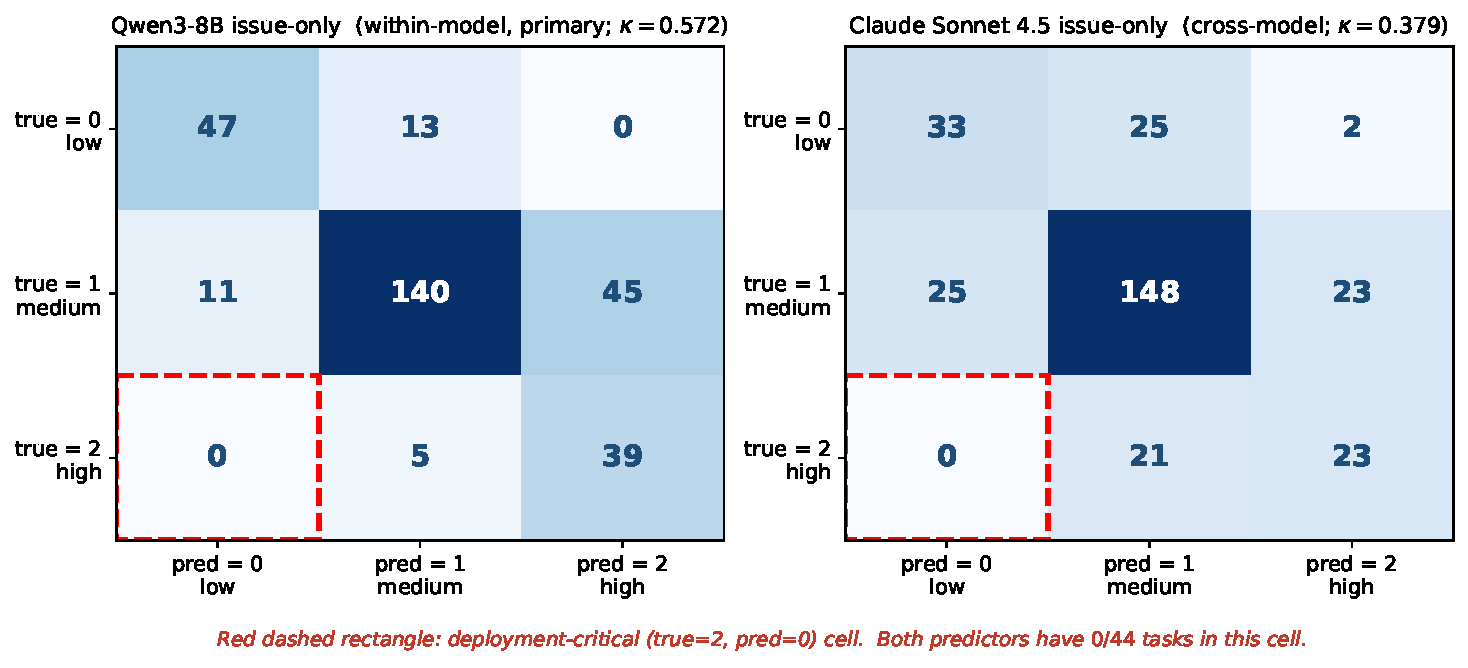
\includegraphics[width=0.95\linewidth]{fig_confusion.pdf}
\caption{\textbf{Predictor confusion matrices} against the LLM-with-patch reference on 300 SWE-bench Lite tasks. Rows denote the reference class and columns denote the predicted class. The deployment-critical under-allocation cell, true class~2 and predicted class~0, is empty for both predictors. The primary Qwen predictor
(left) has higher class-2 recall ($39/44$) than the cross-model Claude predictor (right; $23/44$), but both avoid the high-to-low error that would route a high-consequence task to the lowest compute tier.}
\label{fig:confusion}
\end{figure}

This predictor is imperfect, but its error pattern is useful for deployment. When the
predictor is wrong, it typically errs to an adjacent class, so a high-consequence task is routed at worst to a medium budget rather
than to the cheapest tier. In \S\ref{sec:exp}, we show that this
safety-respecting predictor is sufficient for downstream allocation: on SWE-bench Lite, predictor-driven routing retains most of the gain achieved by oracle-consequence routing under the same compute budget.

\section{Method: Cost-Weighted Compute Allocation}
\label{sec:method}
The previous sections establish that consequence is a measurable,
task-level cost signal distinct from difficulty (\S\ref{sec:cons}), that
current thinking models do not allocate compute by it on their own
(\S\ref{sec:audit}), and that it can be predicted before a task is solved
from issue-level information alone (\S\ref{sec:pred}). Together these make
an explicit scheduling layer both necessary and feasible. We now specify
how that scheduler should use the consequence signal under a fixed
compute budget.

The setup is a multi-tier compute system: a finite set of compute tiers $\{T_1, \ldots, T_K\}$ ordered from cheap to expensive, where each tier is either a different model family, a different sampling temperature, a different self-consistency budget, or a different thinking-token budget on the same model. The deployer has a total compute budget $B$ to spend across a stream of tasks $X$.

\textbf{Objective.} Minimizing the cost-weighted loss on the task stream under a total-compute constraint is
\begin{equation}\label{eq:budgetobj}
\min_{T:\,X\to\{T_1,\dots,T_K\}}\ \sum_{x\in X}\, \mathrm{cost}(x)\cdot
\bigl[\,1 - p\bigl(\text{correct}\mid x, T(x)\bigr)\bigr]
\quad\text{s.t.}\quad
\sum_{x\in X} c(T(x)) \leq B,
\end{equation}
where $c(T_k)$ is the per-task compute price of tier $T_k$. With
$\mathrm{cost}(x){\equiv}1$, Eq.~\ref{eq:budgetobj} reduces to plain
accuracy maximization under a compute budget---the objective implicit in prior adaptive-compute work.

\textbf{Algorithm.} We instantiate Eq.~\ref{eq:budgetobj} with a simple decoupled scheme. Given the predicted consequence $\hat{c}(x) \in \{0,1,2\}$ from \S\ref{sec:pred} and a target overall
compute budget $B$, we sort tasks by $\hat{c}(x)$ in descending order and assign them to compute tiers from premium to cheap until the
budget is exhausted (Algorithm~\ref{alg:cons-route}). In the fixed-quota variants of \S\ref{sec:exp}, the top-$q\%$ tasks by
$\hat{c}$ go to the premium tier and the rest go to the cheap tier;
$q$ is chosen so that total compute matches the difficulty-based baseline. This decoupled scheme assumes a monotone relationship between $\hat{c}$ and the marginal value of more compute---an
assumption we test directly in \S\ref{sec:exp}.

\begin{algorithm}
\caption{Cost-weighted compute allocation}\label{alg:cons-route}
\begin{algorithmic}[1]
\REQUIRE Tasks $X$; predictor $\hat{c}$; tiers $T_1, \ldots, T_K$ with prices $c(T_k)$; total budget $B$.
\STATE Score each task: $s(x) \leftarrow \hat{c}(x)$
\STATE Sort $X$ by $s(\cdot)$ in descending order
\STATE Initialize spent $\leftarrow 0$, $T(x) \leftarrow T_1$ for all $x$
\FOR{$k = K$ down to $2$}
  \FOR{$x$ in sorted order}
    \IF{$T(x) = T_1$ and spent $+ [c(T_k) - c(T_1)] \leq B - \sum_{x'} c(T(x'))$}
      \STATE $T(x) \leftarrow T_k$
      \STATE spent $\leftarrow$ spent $+ [c(T_k) - c(T_1)]$
    \ENDIF
  \ENDFOR
\ENDFOR
\RETURN $T$
\end{algorithmic}
\end{algorithm}

The scheme has three properties worth highlighting. First, it does
not retrain any reasoning model; it sits entirely at the scheduling
layer. Second, the predictor only needs to be ordinal-correct
on the safety dimension---ranking class-2 tasks above class-0 tasks
matters far more than getting the absolute label right. Third, the
scheme degrades gracefully: with a perfect predictor we recover
oracle-consequence routing, with a random predictor we recover random
routing, and with the difficulty score substituted for $\hat{c}$ we
recover the Snell-style difficulty-aware baseline.

\section{Experiments}
\label{sec:exp}

We test Algorithm~\ref{alg:cons-route} on a 16-model SWE-bench
compute-tier benchmark.

\textbf{Setup.} We aggregate the per-task resolution status of 16
public SWE-bench leaderboard solvers spanning four years of model
generations. These include RAG baselines on Claude 2 and GPT-4,
SWE-agent variants on Claude 3 Opus and Claude 3.5 Sonnet, and more
recent agentic systems on Claude 4 Sonnet, including SWE-agent,
ExpeRepair, and KGCompass. We sort the 16 models by total resolved
count and form two tiers: a cheap tier consisting of the bottom
4 models, and a premium tier consisting of the top 4 models.
For each task, $p_{\mathrm{cheap}}(x)$ is the empirical fraction of
cheap-tier solvers that resolve the task. We define
$p_{\mathrm{premium}}(x)$ analogously for the premium tier. Unless
otherwise stated, we assume a compute price ratio
$c(\text{premium})/c(\text{cheap}) = 4$, consistent with typical
model-tier price gaps on commercial APIs. This ratio is an
assumption, not a measurement; at the matched-compute operating
point the strategy comparison is unaffected by it by construction
--- every strategy routes the same number of tasks premium --- and
it only scales the budget axis of the Pareto analysis.

\textbf{Strategies.} We compare seven allocation strategies under a
matched total compute budget. Random routes a uniformly random
top-$q\%$ subset of tasks to the premium tier; it is averaged over
$1{,}000$ random allocations at the same top-$25\%$ premium budget.
Difficulty-aware
(Snell-style~\citep{snell2024scaling}) routes the top-$q\%$ by
outcome-derived difficulty ($1-\overline{\mathrm{passrate}}$ across
the $16$ systems; \S\ref{sec:cons}), the strongest difficulty signal
in this data; deployment-time \emph{predicted}-difficulty variants
are evaluated in \S\ref{sec:whyfail}. Consequence-aware
(predictor) routes the top-$q\%$ by the issue-only consequence
predictor of \S\ref{sec:pred}. We evaluate two predictor variants:
the Qwen issue-only predictor, which is our primary deployment-time
consequence predictor, and the cross-model Claude issue-only predictor,
which serves as a robustness check. Consequence-aware (oracle) replaces the
predictor with the LLM-with-patch label, isolating the upper bound of
a one-signal consequence router. Finally, Priority-aware variants route the top-$q\%$ by
$\hat{c}(x) \cdot [p_{\mathrm{premium}}(x) -
p_{\mathrm{cheap}}(x)]$. This two-signal variant accounts not only
for the cost of an error, but also for whether premium compute changes
the outcome. Because the marginal-gain term
$p_{\mathrm{premium}}(x)-p_{\mathrm{cheap}}(x)$ is computed from
benchmark tier outcomes, we treat the priority-aware variants as
analysis variants rather than fully deployment-time schedulers. A
fully deployment-time priority-aware scheduler would require a
marginal-gain predictor; prompted marginal-gain predictors do not
reliably close this gap (Appendix~\ref{app:marginal}).



\textbf{Metric.} We report cost-weighted loss
\[
\mathcal{L}(T) = \sum_x \mathrm{cons}(x)\cdot
[\,1 - p_{T(x)}(x)\,],
\]
where $\mathrm{cons}(x)$ is the LLM-with-patch consequence label and
$p_{T(x)}(x)$ is the empirical success probability of the tier assigned
to task $x$. The main table reports results on $N=300$ SWE-bench Lite
tasks at a matched-compute operating point where the top-$25\%$ of
tasks are routed to the premium tier.

\begin{table}[t]
\centering
\caption{\textbf{Main results.} Cost-weighted loss $\mathcal{L}$,
relative reduction over the difficulty-aware baseline, and average
accuracy on $N{=}300$ SWE-bench Lite tasks. All strategies are evaluated
at the same compute budget: top-$25\%$ premium routing with a
cheap/premium price ratio of $1{:}4$. Difficulty-aware allocation is
worse than Random at this operating point. The Qwen issue-only consequence router is the primary deployment-time
variant and retains $93.6\%$ of the corresponding consequence-oracle
gain. The priority-aware rows additionally use empirical marginal-gain
information and should be interpreted as an analysis of the extra value
available when marginal gain can be estimated.}
\label{tab:main}
\small
\begin{tabular}{lrrr}
\toprule
Strategy & $\mathcal{L}$ & $\Delta$ vs Diff & Accuracy \\
\midrule
Difficulty-aware (Snell-style)~\citep{snell2024scaling}              & $268.25$ & ~~$0\%$ baseline & $0.054$ \\
Random (mean over $1{,}000$ draws)                                    & $231.20$ & $+13.8\%$ & $0.180$ \\
\midrule
Consequence-aware (Claude issue-only; cross-model)          & $220.50$ & $+17.8\%$ & $0.174$ \\
Consequence-aware (Qwen issue-only; deployment-time)                        & $209.75$ & $+21.8\%$ & $0.184$ \\
Consequence-aware (with-patch oracle)                                            & $205.75$ & $+23.3\%$ & $0.187$ \\
\midrule
Priority-aware (Qwen consequence + empirical marginal gain)  & $\mathbf{186.00}$ & $\mathbf{+30.7\%}$ & $\mathbf{0.274}$ \\
Priority-aware (oracle consequence + empirical marginal gain) & $179.75$ & $+33.0\%$ & $0.278$ \\
\bottomrule
\end{tabular}
\end{table}

\begin{figure}[t]
\centering
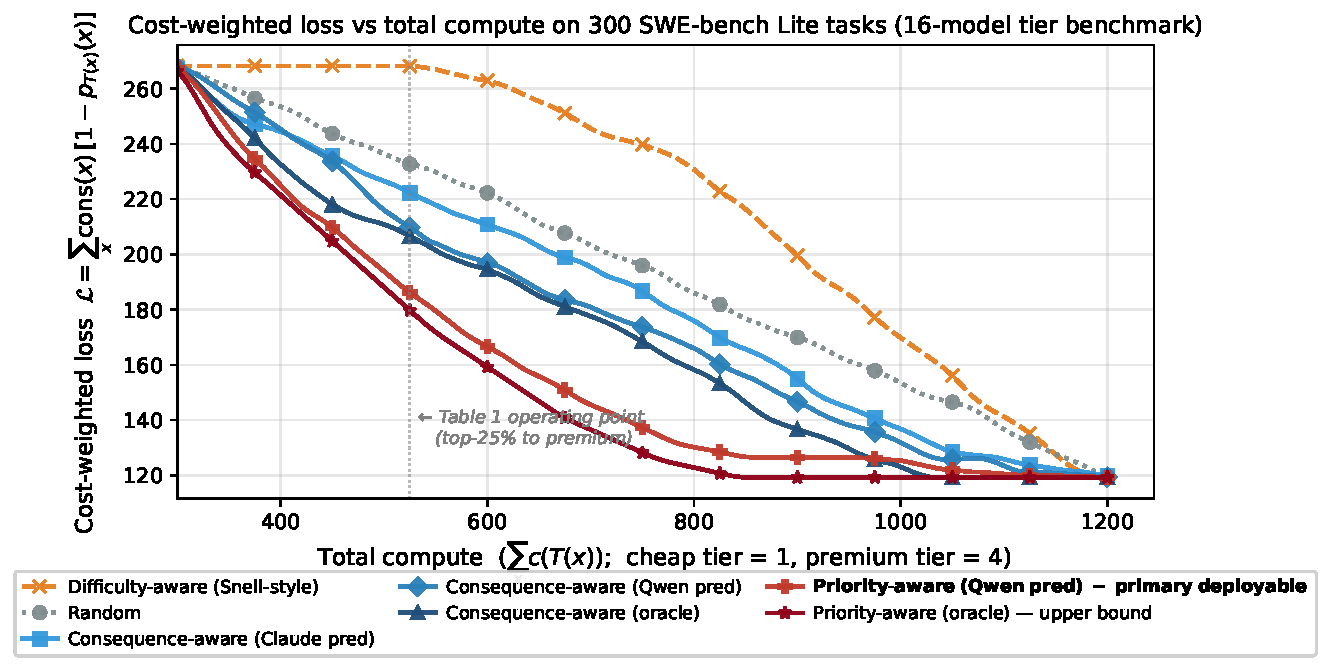
\includegraphics[width=\linewidth]{fig_pareto.pdf}
\caption{\textbf{Pareto curve: cost-weighted loss vs total compute}
on the 16-model SWE-bench compute-tier benchmark. Each curve sweeps
the fraction of tasks routed to the premium tier from $0$ to $100\%$.
The difficulty-aware curve is flat across much of the budget range and
is dominated by the random baseline. This indicates that additional
premium compute spent on the hardest tasks does not reliably reduce
cost-weighted loss, because many of those tasks remain unsolved even
at the premium tier. The priority-aware variants Pareto-dominate all
others, and the version using Qwen issue-only consequence together
with empirical marginal gain closely tracks the corresponding oracle
across the budget axis. The dotted vertical line marks the
top-$25\%$ premium operating point used in Table~\ref{tab:main}.}
\label{fig:pareto}
\end{figure}

\textbf{Consequence-aware allocation improves cost-weighted routing.}
Table~\ref{tab:main} reports the main results at the top-$25\%$
premium operating point, and Figure~\ref{fig:pareto} shows the full
Pareto curve across compute budgets. The Qwen issue-only consequence router is the primary deployment-time
variant. It reduces cost-weighted loss by $21.8\%$ relative to the
difficulty-aware baseline. Its oracle counterpart, which uses the
LLM-with-patch consequence label, reduces loss by $23.3\%$. Thus, the
deployment-time predictor retains $93.6\%$ of the consequence-oracle
gain. This confirms that the safety-respecting issue-only predictor of
\S\ref{sec:pred} translates directly into downstream routing quality
without access to gold patches or benchmark outcome statistics.

\textbf{Empirical marginal-gain information improves routing further.}
When we additionally multiply consequence by empirical marginal gain,
the Qwen-based priority-aware variant reduces cost-weighted loss by
$30.7\%$ at the same compute budget. The corresponding oracle reduces
loss by $33.0\%$, so the Qwen consequence predictor retains $92.9\%$
of the priority-oracle gain under this two-signal analysis. Because
the marginal-gain term is computed from benchmark cheap- and
premium-tier outcomes, we interpret this result as measuring the
potential value of marginal-gain estimation rather than as a fully
deployment-time scheduler.


\textbf{Statistical robustness.} Appendix~\ref{app:bootstrap} reports
task-level bootstrap confidence intervals over $5{,}000$ resamples of
the $300$ SWE-bench Lite tasks. The Qwen issue-only consequence router
remains consistently better than difficulty-aware routing under this
resampling analysis ($95\%$ CI $[+17.6\%, +25.5\%]$), and the ordering
Consequence-aware $>$ Random $>$ Difficulty-aware holds in every
resample. We further perform a leave-one-class-2-out analysis in
Appendix~\ref{app:bootstrap} to verify that the gain is not driven by
a single high-consequence task. Finally, the entire strategy ordering
replicates on a second, disjoint pool of $140$ database/ORM tasks
from SWE-bench Verified~\citep{openai2024swebenchverified} with an
independent $20$-model tier system (Appendix~\ref{app:seconddomain}). When the labeling judge is
replaced with a different model family, difficulty-aware routing
remains worst and priority-aware best on both pools, while the
consequence-only margin over random is judge-dependent: it collapses
when a judge's calibration flattens the cost weights, exactly as the
cost-weighted objective predicts (Appendix~\ref{app:judge2}).

\textbf{Difficulty-aware allocation is worse than random at the main
operating point.} The most striking result in Table~\ref{tab:main} is
that difficulty-aware routing underperforms the random baseline by
$13.8\%$ on average at the top-$25\%$ premium budget. A top-$25\%$ selection
ranked by difficulty captures $0\%$ of the cost-weighted gain available
in the data. In contrast, random selection captures $25\%$
on average,
consequence-only oracle selection captures $43\%$, and priority-oracle
selection captures $59\%$. This suggests that difficulty is not merely
an incomplete routing signal under a cost-weighted objective; at this
operating point, it routes premium compute toward tasks with low
marginal return. The next section analyzes this failure mechanism by
decomposing consequence, difficulty, confidence, and marginal utility.

\section{Why Difficulty-Aware Allocation Fails}
\label{sec:whyfail}

The results of \S\ref{sec:exp} raise a natural question: Why does a
strategy that allocates more compute to harder tasks perform worse than
allocating randomly? We answer this question in two steps. First, we test the alternative interpretation that consequence is merely a re-skinning of cross-model disagreement, and find that consequence contributes substantial additional explanatory power. Second, we
examine per-task marginal utility and show that difficulty is
anti-correlated with where additional compute actually helps.

\subsection{Confounding ablation: consequence is not a proxy of confidence}
\label{sec:p0b}

One might argue that consequence works only because it
inadvertently captures another useful signal, namely cross-model disagreement on a task, which acts as a confidence proxy. To test this alternative, we construct
\[
Y(x) \;=\; \mathrm{cons}(x)\cdot
\bigl[\,p_{\mathrm{premium}}(x) - p_{\mathrm{cheap}}(x)\,\bigr],
\]
the cost-weighted marginal gain of routing task $x$ to the premium
tier. We then ask whether consequence carries information about
$Y(x)$ beyond what is already explained by difficulty and per-task
pass-rate variance. The latter measures how much public solvers
disagree on the task, and serves as our confidence proxy. Controlling
for both difficulty and pass-rate variance, the partial Spearman
correlation remains large:
\[
\rho\bigl(\,\mathrm{cons},\, Y \,\big|\, \mathrm{diff},\,
\mathrm{passvar}\,\bigr) = +0.696,\quad p < 10^{-43}.
\]
A hierarchical regression on $Y(x)$ confirms the same conclusion, as shown in Table~\ref{tab:r2decomp}. Difficulty plus pass-rate variance explains $R^2 = 0.474$, while adding consequence increases this to
$R^2 = 0.738$. This is an absolute gain of $26.4$ percentage points,
or $+55.7\%$ relative. Moreover, difficulty contributes almost no
incremental variance once pass-rate variance is included
($R^2_{\mathrm{diff}+\mathrm{passvar}} -
R^2_{\mathrm{passvar}} = 0.0004$). Thus, the gain of
priority-aware routing in Table~\ref{tab:main} is not produced by
recovering a difficulty or confidence signal in disguise.

\begin{table}[h]
\centering
\caption{\textbf{R\textsuperscript{2} decomposition on the
cost-weighted marginal value $Y$.} $Y$ measures the value of upgrading
a task from the cheap tier to the premium tier after weighting by
consequence. Difficulty alone explains $28\%$ of the variance, and
pass-rate variance, our confidence proxy, explains $47\%$. Adding
consequence on top of both lifts $R^2$ from $0.474$ to $0.738$, an
absolute gain of $26.4$ percentage points ($+55.7\%$ relative).}
\label{tab:r2decomp}
\small
\begin{tabular}{lc}
\toprule
Predictors in linear regression on $Y = \mathrm{cons}\cdot\Delta\mathrm{success}$ & $R^{2}$ \\
\midrule
Difficulty only                                       & $0.281$ \\
Pass-variance only (confidence proxy)                 & $0.474$ \\
Consequence only                                      & $0.350$ \\
Difficulty + Pass-variance                            & $0.474$ \\
Difficulty + Pass-variance + \textbf{Consequence}     & $\mathbf{0.738}$ \\
\midrule
$\Delta R^{2}$ from adding Consequence                & $\mathbf{+0.264}$ \;($+55.7\%$ relative) \\
\bottomrule
\end{tabular}
\end{table}

\begin{figure}[t]
\centering
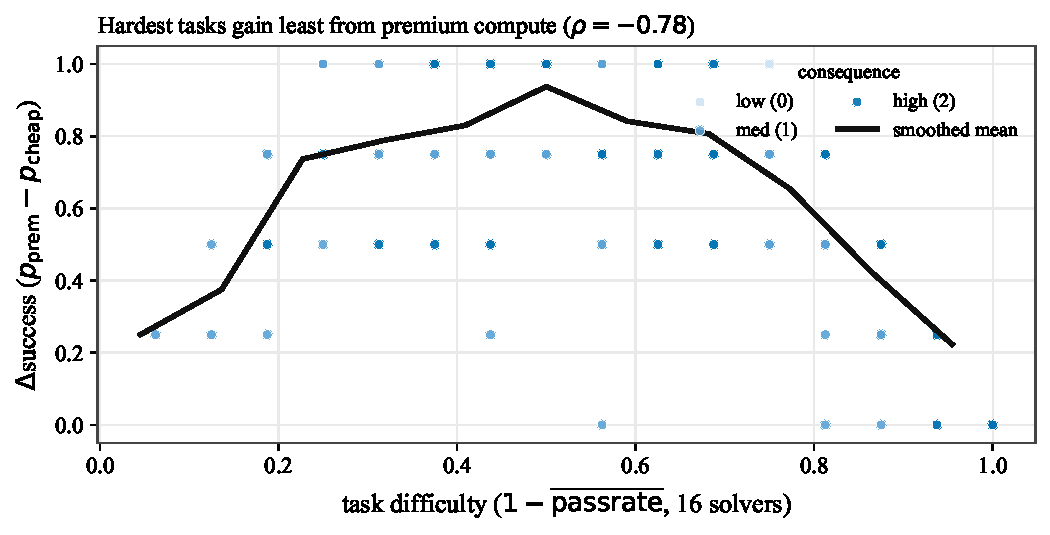
\includegraphics[width=\linewidth]{fig_marginal.pdf}
\caption{\textbf{Why difficulty-aware allocation fails: $\Delta$success
collapses on the hardest tasks.} Each marker is one of the 300
SWE-bench Lite tasks, colored by consequence class. The marginal gain
$\Delta\mathrm{success} = p_{\mathrm{premium}}(x) -
p_{\mathrm{cheap}}(x)$ measures how much accuracy improves when task
$x$ is routed to the premium tier. The binned trend line rises through
the moderate-difficulty region and then collapses on the hardest
tasks, producing a strong negative correlation
($\rho = -0.78$, $p < 10^{-60}$). A scheduler that allocates premium
compute to the difficulty tail therefore spends budget where extra
compute rarely changes the outcome.}
\label{fig:marginal}
\end{figure}

\subsection{Marginal utility: hardest tasks are unsolvable at any tier}
\label{sec:marginal}

Let $\Delta\mathrm{success}(x) = p_{\mathrm{premium}}(x) -
p_{\mathrm{cheap}}(x)$ denote the marginal accuracy gain from upgrading
task $x$ from the cheap tier to the premium tier. This quantity
measures where extra compute changes the outcome. Three observations
explain the failure of difficulty-aware allocation.

\textbf{Difficulty is anti-correlated with marginal gain.}
\(\rho(\mathrm{difficulty}, \Delta\mathrm{success}) = -0.78\)
($p < 10^{-60}$). The hardest tasks are those on which all 16 models
struggle. They are also the tasks where even the premium tier often
does not help. A difficulty-aware scheduler therefore concentrates its
upgrade budget on tasks that cannot be saved by the available premium
tier.

\textbf{How much of this is mechanical?} Difficulty and
$\Delta\mathrm{success}$ are computed from the same outcomes, and a
task solved by no system has $\mathrm{difficulty} = 1$ and
$\Delta\mathrm{success} = 0$ \emph{by identity}, so the never-solved
floor contributes a negative component by construction. We decompose
this. Excluding the $76/300$ never-solved tasks, the correlation
remains strong ($\rho = -0.489$, $p < 10^{-14}$): among tasks that at
least one system solves, harder tasks genuinely benefit less from the
premium tier. (On the Verified pool the coupling is mostly the floor
identity: $-0.377 \to -0.043$, n.s., after excluding its $18$ floor
tasks.) We additionally measured the relationship with a fully
independent, deployment-time difficulty estimate --- issue-only
solvability forecasts from two model families
(Appendix~\ref{app:marginal}) --- which correlates with
$\Delta\mathrm{success}$ at $|\rho| < 0.15$ (n.s.) in every
family$\times$pool combination.

\textbf{What this means for difficulty routing.} Routing by
outcome-derived difficulty --- the strongest available version, and
the one in Table~\ref{tab:main} --- is worse than random because it
actively selects the unsalvageable floor. Routing by the
deployment-time \emph{predicted} difficulty removes the mechanical
component along with most of the signal, and lands at the level of
random ($+12.4\%$ to $+16.7\%$ vs.\ random's $+13.8\%$ on Lite;
$+9.4\%$ to $+12.9\%$ vs.\ $+12.4\%$ on Verified) --- consistently
below consequence routing ($+21.8\%$ / $+14.9\%$). The comparison is
ironic but informative: the better difficulty is measured, the worse
difficulty routing performs, because true difficulty anti-selects
marginal gain. Difficulty routing at its noisiest matches random; at
its most informed, it is worse; in no variant does it match or
exceed consequence routing.

\textbf{Consequence is uncorrelated with marginal gain.}
\(\rho(\mathrm{cons}, \Delta\mathrm{success}) = +0.09\) (n.s.).
Consequence does not predict whether extra compute will help on a
given task. Instead, it predicts whether that help would be valuable
if it occurs.

\textbf{Consequence and marginal gain combine multiplicatively.}
The priority signal
\[
\mathrm{priority}(x)
=
\mathrm{cons}(x)\cdot\Delta\mathrm{success}(x)
\]
ranks tasks by their cost-weighted return on extra compute. This
decomposition matches the empirical ordering in Table~\ref{tab:main}:
priority-aware routing performs best, followed by consequence-only
routing, random routing, and finally difficulty-aware routing. At the
top-$25\%$ premium operating point, a priority ranking captures
$59\%$ of the total cost-weighted gain available in the data. A
consequence-only ranking captures $43\%$, random selection captures
$25\%$ on average, and difficulty ranking captures $0\%$. The gap between
consequence-only and priority-aware routing is meaningful, but not
transformative. This is consistent with the $+21.8\%$ versus
$+30.7\%$ loss reduction observed in Table~\ref{tab:main}.

Together, these observations explain the negative result for
difficulty-aware allocation. A cost-blind scheduler that spends more
compute on harder tasks spends its budget where extra compute has the
lowest marginal return. Figure~\ref{fig:marginal} visualizes this
effect. $\Delta\mathrm{success}$ rises with difficulty up to the
moderate range and then collapses on the unsolvable tail, producing the strongly negative Spearman correlation. Appendix~\ref{app:marginal} reports the per-task view: the top-ranked tasks by priority have moderate difficulty and large $\Delta\mathrm{success}$, whereas the
top-ranked tasks by difficulty all have $\Delta\mathrm{success}=0$.

\section{Discussion and Limitations}
\label{sec:discussion}

\textbf{Is cost-weighted evaluation circular?} A natural objection
is that consequence-aware routing is evaluated on a loss weighted by
the same labels it routes on, making the oracle rows favorable by
construction. Three observations separate our claims from this
tautology. First, the deployment-relevant result is not
oracle-vs-uniform but predictor-vs-oracle: an issue-only predictor
that never sees the realized fix recovers $93.6\%$ of the oracle
gain, an empirical fact about predictability rather than a
restatement of the objective. Second, the headline negative result
--- difficulty-aware routing losing to random --- makes no reference
to consequence weights at all in its mechanism
($\rho(\mathrm{difficulty}, \Delta\mathrm{success}) = -0.78$), and
persists under all five cost mappings of Appendix~\ref{app:costmap}
and under labels produced by an independent judge from a different
model family (Appendix~\ref{app:judge2}). Third, any deployed
scheduler must adopt \emph{some} error-cost weighting~\citep{sayin2025rethinking}; uniform
weighting is itself a choice --- the one implicitly made by
accuracy-maximizing allocation --- and our results quantify what that
implicit choice forgoes when real error costs are heterogeneous.
Finally, the framework makes falsifiable predictions about when its
advantage should \emph{disappear}, and the out-of-domain probe of
Appendix~\ref{app:ood} confirms them.

\textbf{Construct validity of consequence.} Throughout the main text,
the primary consequence label is produced by an LLM judge that observes
the issue, the gold patch, and the modified files. This choice gives
the judge access to the realized fix, but it also raises a construct
validity concern: the label should reflect a human-interpretable notion
of deployment harm rather than an artifact of the LLM judge. To address
this, we conduct a three-annotator human study on a $150$-task
stratified sample drawn from SWE-bench Lite and Multi-SWE-bench mini
(Appendix~\ref{app:iaa}). The annotators apply the rubric consistently,
and the LLM-with-patch judge agrees with the human majority at
$\kappa = 0.50$. More importantly, the central orthogonality result of
\S\ref{sec:cons} replicates under human labeling
($\rho = -0.066$, n.s.). We therefore use the human labels as a
construct-validity check, while retaining the LLM-with-patch label as
the primary signal in the main experiments because it covers the full
SWE-bench Lite task pool.

\textbf{Scope of evaluation.} Our main allocation experiment uses
publicly available per-task outcomes from 16 SWE-bench Lite leaderboard
solvers. This design allows us to compare many compute tiers on the
same task set and to estimate per-task marginal gains from upgrading
cheap models to premium models. However, it is still an offline
compute-tier study rather than a fully controlled intervention on a
single reasoning model. As controlled supporting evidence, Appendix~\ref{app:within} repeats
the allocation experiment with a single fixed Claude Sonnet~4.5 agent,
varying only test-time compute (oracle best-of-$k$ attempts). The same qualitative ordering is reproduced: consequence-aware and
priority-aware routing beat the difficulty-aware baseline, which is
again worse than random. Appendix~\ref{app:seconddomain} further
repeats the full allocation comparison on a consequence-rich pool of
$140$ database/ORM tasks from SWE-bench Verified ($33.6\%$ class-$2$)
with an independent $20$-model tier system, and the strategy ordering
replicates exactly. Appendix~\ref{app:ood} further probes a
non-software domain --- business-database analytics (BIRD
text-to-SQL~\citep{li2023bird}) --- with a fully end-to-end pipeline (live two-tier
inference, execution grading, predictor routing), finding that the
framework's predictions track the domain's cost structure: the pool
lacks the cost heterogeneity and the negative difficulty--gain
coupling that drive the main result, and correspondingly consequence
routing collapses to random there while difficulty routing is no
longer penalized. Broader multi-domain evaluation remains future
work.

\textbf{Cost is a coarse scalar.} We represent consequence as an
ordinal label in $\{0,1,2\}$. This is a deliberate simplification.
Real deployment cost is multidimensional, including financial,
reputational, safety, privacy, and regulatory harms, and the same bug
may have different consequences in different production contexts. Our
labels should therefore be interpreted as a coarse ordering of
deployment harm, not as calibrated monetary costs. The framework in
Eq.~\ref{eq:budgetobj} naturally extends to richer cost models,
including continuous costs or task-dependent cost vectors. The
three-class version used here is intended as a minimal instantiation
that current LLM judges and human annotators can apply reliably from
issue text and patches. Appendix~\ref{app:costmap} verifies that the
qualitative ordering of routing strategies remains stable under
several monotone cost mappings, including $\{1,2,3\}$, $\{1,2,5\}$,
and $\{1,3,10\}$.

\textbf{Marginal-gain estimation.} The primary deployment-time
scheduler in this paper uses only the issue-only consequence predictor.
The priority-aware variants additionally use empirical marginal gain,
computed from observed cheap- and premium-tier success rates in the
benchmark; they are analysis upper bounds, not deployable schedulers.
We tested the most accessible deployment-time route --- prompting two
model families to forecast cheap-tier and frontier-tier success from
the issue text (Appendix~\ref{app:marginal}): absolute success levels
are moderately predictable ($\rho$ up to $+0.39$), but their
difference, the marginal gain, is not ($|\rho| < 0.07$, n.s., in
all family$\times$pool combinations), and the resulting
deployment-time priority scheduler does not reliably beat
consequence-only routing. Estimating the value of additional
computation appears to be the genuinely hard half of the problem;
learning it from execution feedback, model confidence, agent traces,
or early attempts remains an important direction for future work.

\section{Conclusion}

Adaptive test-time compute methods for reasoning models have largely
optimized average accuracy under a compute budget. We argue that this
objective is incomplete for deployment: tasks differ not only in how
hard they are, but also in how costly their errors would be. The
missing signal is per-task consequence. We show that consequence is
measurable, distinct from difficulty and confidence, predictable from
issue text alone, and usable as a routing signal without retraining the
reasoning model.

On a 16-model SWE-bench compute-tier benchmark, the fully
deployment-time consequence-only router reduces cost-weighted loss by
$21.8\%$ relative to difficulty-aware routing. A priority-aware variant that additionally uses empirical marginal gain reaches a $30.7\%$ reduction, showing the potential value of
estimating where extra compute changes the outcome. 
We also find that difficulty-aware routing can underperform random allocation, because the hardest tasks often remain unsolved at every available tier and therefore have low marginal return from extra compute.

These results suggest that test-time compute allocation should not be
treated only as a question of task difficulty. For deployment, the
central question is also what happens if the model is wrong, and
whether extra computation is likely to prevent that error.

\bibliography{references}
\bibliographystyle{plainnat}

\appendix

\section{Human-Label Robustness Check}
\label{app:iaa}

This appendix re-runs two headline checks---consequence--difficulty
orthogonality (\S\ref{sec:cons}) and predictor agreement
(\S\ref{sec:pred})---with consequence labels supplied by a human
majority rather than by an LLM judge. The goal is to verify that the
LLM-based labels used in the main text track a human-interpretable
notion of deployment consequence.

\paragraph{Study design.} We sampled $150$ unique tasks, stratified by
the LLM-with-patch consequence label, drawn $75$ from SWE-bench Lite
and $75$ from Multi-SWE-bench mini. Each annotator's sheet contained
$165$ rows in a randomized order, with $15$ hidden duplicates (five
per class) used to measure self-consistency. Three annotators
participated: one of the authors, one CS PhD outside the project, and
one non-author CS graduate student; none had access to the gold patch,
the file diff, or each other's labels. Each annotator first completed
a $9$-task calibration warm-up with reference labels before the
$165$-task evaluation.

\paragraph{Annotators apply the rubric consistently.} Each annotator's
self-consistency is measured by Cohen's $\kappa$ on the $15$ hidden
duplicates: two annotators are perfectly self-consistent
($\kappa = 1.000$, $100\%$ raw agreement) and the third reaches
$\kappa = 0.789$ ($86.7\%$). The rubric is internally consistent
within each annotator.

\paragraph{Orthogonality replicates under human labels.} On the $75$
SWE-bench Lite tasks for which we have both human-majority labels and
the difficulty estimate of \S\ref{sec:cons},
\[
\rho\bigl(\mathrm{human}\!-\!\mathrm{cons},\ \mathrm{difficulty}\bigr) = -0.066,\quad p = 0.57.
\]
The central orthogonality result of \S\ref{sec:cons} \textbf{replicates}
under human labeling: consequence is statistically independent of
difficulty whether the label is produced by a rule, by an LLM shown
the gold patch, by an LLM shown only the issue, or by a human
majority of three independent annotators
(see Appendix~\ref{app:rubric} for the full four-labeling comparison).

\paragraph{LLM labels agree with human majority.}
Table~\ref{tab:human-vs-llm} compares the human majority label against
the three labeling pipelines used in the main text. The LLM-with-patch
judge agrees with the human majority at Cohen's $\kappa = 0.500$, and
the issue-only predictor at $\kappa = 0.517$. The rule-based labeler
agrees at $\kappa = 0.223$, consistent with its purely lexical
construction. Both LLM pipelines pick up the same construct as the
human majority to a moderate degree, supporting their use as the
primary labels in the main text.

\begin{table}[h]
\centering
\caption{Cohen's $\kappa$ between the human majority label and each of
the labeling pipelines used in the main text, on the $75$ SWE-bench
Lite tasks of this study.}
\label{tab:human-vs-llm}
\small
\begin{tabular}{lc}
\toprule
Pipeline & $\kappa$ vs human majority \\
\midrule
Rule-based labeler                       & $0.223$ \\
LLM-with-patch judge (Qwen2.5-7B-Instruct) & $0.500$ \\
LLM-issue-only predictor (Qwen2.5-7B-Instruct) & $0.517$ \\
\bottomrule
\end{tabular}
\end{table}

\paragraph{Final human labels.} We resolve each of the $150$ tasks by
majority vote of the three annotators. $142$ tasks have a clear
majority ($\geq 2$ of $3$ votes); the remaining $8$ are three-way
splits and are conservatively assigned to the middle class. The
resulting class distribution is $\{0{:}45,\ 1{:}67,\ 2{:}38\}$. These
human-majority labels are the basis for the $\rho = -0.066$ result
above and for the corresponding row of Appendix~\ref{app:rubric}'s
four-labeling ablation.

\section{Rubric Ablation: All Four Labelings Give the Same Conclusion}
\label{app:rubric}

A natural reviewer concern is that the central results of the paper
might be artefacts of the specific labeling pipeline used in the main
text (LLM-with-patch). This appendix re-runs two headline analyses---consequence--difficulty
orthogonality (\S\ref{sec:cons}) and matched-compute allocation gain
(\S\ref{sec:exp})---separately under each of the four labelings of the
rubric, and shows that the conclusions are stable.

\textbf{Consequence--difficulty orthogonality replicates under every labeling.}
Table~\ref{tab:abl-ortho} reports $\rho(\mathrm{consequence}, \mathrm{difficulty})$
under the four labeling pipelines. None of the four correlations
reaches significance at $\alpha = 0.05$, and all four are within
$\pm 0.11$ of zero. The construct is statistically independent of
difficulty regardless of who or what produces the label.

\begin{table}[h]
\centering
\caption{\textbf{Rubric ablation — orthogonality.} Spearman
$\rho(\mathrm{consequence}, \mathrm{difficulty})$ on SWE-bench Lite
under each of the four labelings.}
\label{tab:abl-ortho}
\small
\begin{tabular}{lccc}
\toprule
Labeling pipeline & $n$ & $\rho$ & $p$ \\
\midrule
Rule-based                                  & $300$ & $+0.047$ & $0.42$ \\
LLM-with-patch  (Qwen2.5-7B-Instruct; paper primary)   & $300$ & $-0.096$ & $0.10$ \\
LLM-issue-only  (Qwen2.5-7B-Instruct predictor)        & $300$ & $-0.109$ & $0.06$ \\
Human majority  (3-annotator study)         & $\phantom{0}75$  & $-0.066$ & $0.57$ \\
\bottomrule
\end{tabular}
\end{table}

\textbf{Allocation gain replicates under every labeling.}
Table~\ref{tab:abl-gain} re-runs the matched-compute experiment of
\S\ref{sec:exp} four times: in each row, the indicated labeling is
substituted both as the oracle routing signal and as the weight
$\mathrm{cons}(x)$ used in computing the cost-weighted loss. The
priority-aware oracle beats the difficulty-aware baseline by between
$+30.8\%$ and $+36.3\%$ across all four labelings, with the human
labels giving the largest improvement on the 75-task subset they
cover. The robustness of the $30\%+$ priority-aware oracle gain is therefore
not a property of the LLM-with-patch labeler specifically; it reflects
the consequence rubric across multiple independent labelings.

\begin{table}[h]
\centering
\caption{\textbf{Rubric ablation — allocation gain.} Cost-weighted loss
$\mathcal{L}$ at the matched-compute operating point (top-$25\%$ to
the premium tier) on the 16-model SWE-bench compute-tier benchmark,
recomputed four times---once per labeling pipeline---using that
labeling both as the oracle routing signal and as the consequence
weight in $\mathcal{L}$. ``$\Delta$ vs Diff'' is the relative
reduction in $\mathcal{L}$ achieved by the priority-aware oracle
relative to the difficulty-aware (Snell-style) baseline within the
same labeling.}
\label{tab:abl-gain}
\small
\begin{tabular}{lrrrrrr}
\toprule
Oracle labeling & $n$ & Diff & Random & Cons-oracle & Priority-oracle & $\Delta$ vs Diff \\
\midrule
Rule-based                                & $300$ & $406.2$ & $352.5$ & $330.8$ & $\mathbf{281.2}$ & $+30.8\%$ \\
LLM-with-patch (paper main)        & $300$ & $268.2$ & $233.8$ & $205.8$ & $\mathbf{179.8}$ & $+33.0\%$ \\
LLM-issue-only (predictor)         & $300$ & $307.5$ & $266.2$ & $229.5$ & $\mathbf{201.5}$ & $+34.5\%$ \\
Human majority (75 SWE tasks)      & $\phantom{0}75$  & $\phantom{0}75.8$  & $\phantom{0}67.5$  & $\phantom{0}55.2$  & $\phantom{00}\mathbf{48.2}$  & $+36.3\%$ \\
\bottomrule
\end{tabular}
\end{table}

The fact that the rule-based labeler---which is just a hand-written
lexical pattern matcher---and the human-majority labeler---which never
sees an LLM---both yield $30\%+$ priority-aware improvements makes it
unlikely that the gain is simply something the LLM judge invented. The
remainder of the paper retains the LLM-with-patch label as the
primary signal in the main results because it is the labeling under
which all four supporting analyses
(\S\ref{sec:cons}, \S\ref{sec:pred}, \S\ref{sec:exp}, \S\ref{sec:whyfail})
are jointly applicable on the full 300-task pool.

\section{Statistical Robustness of Allocation Results}
\label{app:bootstrap}

This appendix quantifies the statistical stability of the allocation
results in Table~\ref{tab:main}, which are computed on $300$ SWE-bench
Lite tasks of which only $44$ are high-consequence. We report three
complementary analyses: task-level bootstrap confidence intervals, the
variability of the random baseline across allocation draws, and a
leave-one-class-2-out analysis.

\paragraph{Task-level bootstrap confidence intervals.} We resample the
$300$ tasks with replacement $5{,}000$ times and recompute every
strategy's cost-weighted loss and its relative reduction over
difficulty-aware routing at the same top-$25\%$ matched-compute
operating point. Table~\ref{tab:bootstrap} reports $95\%$ percentile
intervals. Every consequence-based strategy improves on
difficulty-aware routing in all $5{,}000$ resamples, and the ordering
Consequence-aware (Qwen) $>$ Random $>$ Difficulty-aware, as well as
Priority-aware $>$ Consequence-aware, holds in $100\%$ of resamples.
For the Random row, the bootstrap resamples tasks while holding one
representative allocation draw fixed; variability across allocation
draws is quantified separately below.

\begin{table}[h]
\centering
\caption{\textbf{Task-level bootstrap} over $5{,}000$ resamples of the
$300$ SWE-bench Lite tasks at the top-$25\%$ matched-compute operating
point. Point estimates match Table~\ref{tab:main}; intervals are
$2.5$--$97.5$ percentile ranges over resamples.}
\label{tab:bootstrap}
\small
\resizebox{\linewidth}{!}{%
\begin{tabular}{lrrrr}
\toprule
Strategy & $\mathcal{L}$ & $95\%$ CI ($\mathcal{L}$) & $\Delta$ vs Diff & $95\%$ CI ($\Delta$) \\
\midrule
Difficulty-aware                                   & $268.25$ & $[249.2,\,286.8]$ & baseline   & --- \\
Random (mean over $1{,}000$ draws)                 & $231.20$ & $[214.8,\,251.2]$ & $+13.8\%$  & $[+9.9\%,\,+16.2\%]$ \\
Consequence-aware (Claude issue-only)              & $220.50$ & $[201.2,\,239.8]$ & $+17.8\%$  & $[+14.1\%,\,+21.5\%]$ \\
Consequence-aware (Qwen issue-only)                & $209.75$ & $[190.8,\,230.0]$ & $+21.8\%$  & $[+17.6\%,\,+25.5\%]$ \\
Consequence-aware (with-patch oracle)              & $205.75$ & $[187.0,\,223.8]$ & $+23.3\%$  & $[+19.2\%,\,+27.4\%]$ \\
Priority-aware (Qwen + empirical marginal gain)    & $186.00$ & $[169.5,\,203.0]$ & $+30.7\%$  & $[+27.7\%,\,+33.4\%]$ \\
Priority-aware (oracle + empirical marginal gain)  & $179.75$ & $[163.0,\,197.5]$ & $+33.0\%$  & $[+30.3\%,\,+35.4\%]$ \\
\bottomrule
\end{tabular}%
}
\end{table}

\paragraph{Random baseline across allocation draws.} At the fixed task
set, we draw $1{,}000$ independent random top-$25\%$ allocations. The
cost-weighted loss has mean $231.20$, standard deviation $3.70$, and a
$95\%$ interval of $[224.0,\,238.2]$; every one of the $1{,}000$ draws
outperforms difficulty-aware routing ($268.25$). The Random row of
Table~\ref{tab:main} therefore reports this mean rather than a single
draw.

\paragraph{Leave-one-class-2-out analysis.} Because cost-weighted loss
depends strongly on the $44$ high-consequence tasks, we recompute the
main strategies $44$ times, each time removing one class-2 task. The
reduction over difficulty-aware routing for the Qwen issue-only
consequence router stays within $[+21.5\%,\,+22.3\%]$ (mean
$+21.9\%$) and beats difficulty-aware routing in all $44$ runs; the
priority-aware variant stays within $[+30.3\%,\,+30.9\%]$ (mean
$+30.7\%$), also winning in all $44$ runs. No single high-consequence
task drives the result.

\section{Cost-Mapping Sensitivity}
\label{app:costmap}

The main text maps the ordinal consequence classes $\{0,1,2\}$
directly to scalar weights $\{0,1,2\}$ in the cost-weighted loss. This
appendix verifies that the qualitative conclusions do not depend on
this particular spacing. We recompute the matched-compute allocation
comparison under five monotone cost mappings, applying each mapping
consistently both to the loss weights and to the consequence-based
routing scores. Table~\ref{tab:costmap} reports the results: under
every mapping, the ordering Consequence-aware (Qwen) $>$ Random $>$
Difficulty-aware and Priority-aware $>$ Consequence-aware is
preserved. The Qwen issue-only router's reduction over
difficulty-aware routing ranges from $+17.7\%$ (mapping $\{1,2,3\}$)
to $+29.9\%$ (mapping $\{0,1,5\}$); steeper mappings, which weight
high-consequence errors more heavily, generally favor
consequence-based routing more strongly.

\begin{table}[h]
\centering
\caption{\textbf{Cost-mapping sensitivity.} Cost-weighted loss (and
reduction vs.\ difficulty-aware) at the top-$25\%$ matched-compute
operating point under five monotone mappings of the consequence
classes $\{0,1,2\}$ to scalar weights. The Random column uses one
representative fixed draw for comparability across mappings. The
strategy ordering is preserved under every mapping.}
\label{tab:costmap}
\small
\resizebox{\linewidth}{!}{%
\begin{tabular}{lrrrrrr}
\toprule
Mapping & Diff & Random & Cons-Qwen & Cons-oracle & Pri-Qwen & Pri-oracle \\
\midrule
$\{0,1,2\}$  & $268.2$  & $233.0$ & $209.8$ ($+21.8\%$) & $205.8$ ($+23.3\%$) & $186.0$ ($+30.7\%$) & $179.8$ ($+33.0\%$) \\
$\{1,2,3\}$  & $552.0$  & $482.0$ & $454.5$ ($+17.7\%$) & $449.8$ ($+18.5\%$) & $398.2$ ($+27.9\%$) & $393.2$ ($+28.8\%$) \\
$\{1,2,5\}$  & $634.0$  & $551.5$ & $497.5$ ($+21.5\%$) & $486.2$ ($+23.3\%$) & $448.2$ ($+29.3\%$) & $435.2$ ($+31.3\%$) \\
$\{1,3,10\}$ & $1025.2$ & $888.8$ & $771.8$ ($+24.7\%$) & $746.8$ ($+27.2\%$) & $697.0$ ($+32.0\%$) & $672.8$ ($+34.4\%$) \\
$\{0,1,5\}$  & $391.2$  & $337.2$ & $274.2$ ($+29.9\%$) & $260.5$ ($+33.4\%$) & $249.5$ ($+36.2\%$) & $236.5$ ($+39.6\%$) \\
\bottomrule
\end{tabular}%
}
\end{table}

\paragraph{Continuous severity weights.} The mappings above are still
three-level. To test whether the conclusions depend on discretization
at all, we elicited a rubric-anchored \emph{continuous} severity score
($0$--$100$) for every task, with the gold patch visible, from two
judge families (\texttt{deepseek-chat} and GPT-4o), on both SWE
pools. The continuous scores track the ordinal label
($\rho = 0.38$--$0.49$ across the four judge$\times$pool
combinations) and each other (cross-judge Spearman $0.50$ on Lite,
$0.40$ on Verified), and correlate with difficulty only mildly
($\rho$ between $-0.11$ and $+0.36$). Re-running the full allocation
comparison with the continuous scores as \emph{both} the loss weights
and the oracle routing signal --- while the deployment-time route
remains the unchanged ordinal issue-only predictor --- preserves the
complete strategy ordering in all four combinations
(Table~\ref{tab:contcost}). The paper's conclusions are not an
artifact of the three-class discretization.

\begin{table}[h]
\centering
\caption{\textbf{Allocation under continuous $0$--$100$ severity
weights} from two independent judge families, both pools
(reduction vs.\ difficulty-aware routing; deployment route = ordinal
issue-only predictor throughout). The discrete-table ordering is
preserved in every combination.}
\label{tab:contcost}
\small
\resizebox{\linewidth}{!}{%
\begin{tabular}{llrrrrr}
\toprule
Pool & Weights & Random & Cons-pred & Cons-oracle$_{\mathrm{cont}}$ & Pri-pred & Pri-oracle$_{\mathrm{cont}}$ \\
\midrule
Lite & deepseek-chat & $+13.1\%$ & $+16.7\%$ & $+20.6\%$ & $+25.3\%$ & $+31.5\%$ \\
Lite & GPT-4o        & $+13.9\%$ & $+17.8\%$ & $+20.8\%$ & $+27.6\%$ & $+30.7\%$ \\
Verified & deepseek-chat & $+12.5\%$ & $+14.2\%$ & $+18.7\%$ & $+26.4\%$ & $+30.9\%$ \\
Verified & GPT-4o        & $+13.7\%$ & $+13.8\%$ & $+22.6\%$ & $+25.2\%$ & $+30.1\%$ \\
\bottomrule
\end{tabular}%
}
\end{table}

\section{Predictor Calibration Details}
\label{app:predictor}

This appendix expands \S\ref{sec:pred} with full per-class metrics and
confusion matrices for both predictors evaluated against the
LLM-with-patch reference on all $N{=}300$ SWE-bench Lite tasks. The
class distribution of the with-patch reference is
$\{0{:}60,\ 1{:}196,\ 2{:}44\}$.

\textbf{Primary predictor: Qwen2.5-7B-Instruct issue-only.} Cohen's
$\kappa = 0.572$; class-2 recall $= 88.6\%$ ($39/44$). The confusion
matrix is:
\[
\begin{array}{c|ccc|c}
& \hat{c}{=}0 & \hat{c}{=}1 & \hat{c}{=}2 & \text{total} \\\hline
c{=}0 & 47  & 13  & 0  & 60  \\
c{=}1 & 11  & 140 & 45 & 196 \\
c{=}2 & 0   & 5   & 39 & 44  \\\hline
\text{total} & 58 & 158 & 84 & 300
\end{array}
\]
Per-class precision/recall/F1: class~0 ($0.81/0.78/0.80$), class~1
($0.89/0.71/0.79$), class~2 ($0.46/0.89/0.61$). The deployment-critical severe under-allocation error is zero:
$[2,0]=0$, meaning no high-consequence task is predicted as low
consequence. The opposite extreme error is also zero, $[0,2]=0$,
which means no low-consequence task is escalated to the highest
consequence class. Thus, the total low--high disagreement rate is
$0/300 = 0.0\%$.

\textbf{Cross-model robustness predictor: Claude Sonnet~4.5
issue-only.} Cohen's $\kappa = 0.379$; class-2 recall $= 52.3\%$
($23/44$). The confusion matrix is:
\[
\begin{array}{c|ccc|c}
& \hat{c}{=}0 & \hat{c}{=}1 & \hat{c}{=}2 & \text{total} \\\hline
c{=}0 & 33 & 25 & 2 & 60 \\
c{=}1 & 25 & 148 & 23 & 196 \\
c{=}2 & 0 & 21 & 23 & 44 \\\hline
\text{total} & 58 & 194 & 48 & 300
\end{array}
\]
Per-class precision/recall/F1: class~0 ($0.57/0.55/0.56$), class~1
($0.76/0.76/0.76$), class~2 ($0.48/0.52/0.50$). Despite a noticeably
lower aggregate $\kappa$ than the within-model predictor, the
class-2$\to$class-0 cell still holds at zero. The two low--high
disagreements occur in the conservative direction, class-0$\to$class-2:
they may waste compute, but they do not under-allocate high-consequence
tasks. This supports the conclusion that both predictors avoid the
deployment-critical high-to-low error on this benchmark.

\paragraph{Operating characteristics of the ordinal predictor.} The
three-class predictor admits two alarm thresholds for detecting true
class-$2$ tasks: flag on $\hat{c}{=}2$, or flag on
$\hat{c}{\ge}1$. Across the four pools:

\begin{center}
\small
\begin{tabular}{lcccc}
\toprule
Pool & true $2$s & recall / precision ($\hat{c}{=}2$) & recall / precision ($\hat{c}{\ge}1$) \\
\midrule
Lite      & $44$ & $0.89$ / $0.46$ & $1.00$ / $0.18$ \\
MSWE mini & $3$  & $1.00$ / $0.16$ & $1.00$ / $0.01$ \\
Verified  & $47$ & $0.96$ / $0.62$ & $1.00$ / $0.37$ \\
BIRD      & $3$  & $1.00$ / $0.20$ & $1.00$ / $0.03$ \\
\bottomrule
\end{tabular}
\end{center}

The recall-heavy behavior is an operating-point choice appropriate to
asymmetric error costs, not an accident, and its false-alarm price is
internal to every allocation number we report. The operating point is
also not a knife edge: eliciting a \emph{continuous} issue-only
severity score ($0$--$100$) from two independent model families yields
a threshold-sweepable class-$2$ detector with AUC $0.69$--$0.82$
across judge$\times$pool combinations, on which recall $\ge 0.9$ is
available across a wide threshold band (e.g., deepseek-chat at
thresholds $50$--$70$: recall $0.91$--$0.98$ at precision
$0.41$--$0.45$ on Verified). On the safety
property: across the four pools the predictor has missed $0$ of $97$
true high-consequence tasks; the one-sided $95\%$ Clopper--Pearson
upper bound on the miss rate is $3.0\%$, which is the honest
quantitative content of the ``never misclassifies'' statement.

\section{Per-Task Marginal Utility (Excerpt)}
\label{app:marginal}

This appendix supports \S\ref{sec:marginal} with a per-task view of
the priority signal
$\mathrm{priority}(x) = \mathrm{cons}(x) \cdot
\Delta\mathrm{success}(x)$. The complete per-task table (all $300$
rows) is included with the submission as a supplementary CSV;
Table~\ref{tab:marg} below shows the top eight tasks by priority and
the top four tasks by raw difficulty for contrast.

\begin{table}[h]
\centering
\caption{Per-task marginal utility excerpt. Top eight tasks by
priority $= \mathrm{cons}\cdot\Delta\mathrm{success}$ and top four
tasks by difficulty $= 1 - \overline{\mathrm{passrate}}$. The
priority-ranked tasks all have moderate difficulty and large
$\Delta\mathrm{success}$; the difficulty-ranked tasks all have
$\Delta\mathrm{success} \approx 0$ (premium tier cannot solve them
either), so allocating extra compute to them returns zero
cost-weighted gain.}
\label{tab:marg}
\small
\begin{tabular}{lcccc}
\toprule
Selection & cons & difficulty & $\Delta$success & priority \\
\midrule
\multicolumn{5}{l}{\textit{Top-8 by priority}} \\
top-1 & $2$ & $0.50$ & $1.00$ & $2.00$ \\
top-2 & $2$ & $0.50$ & $1.00$ & $2.00$ \\
top-3 & $2$ & $0.56$ & $0.75$ & $1.50$ \\
top-4 & $2$ & $0.56$ & $0.75$ & $1.50$ \\
top-5 & $2$ & $0.62$ & $0.75$ & $1.50$ \\
top-6 & $2$ & $0.62$ & $0.75$ & $1.50$ \\
top-7 & $1$ & $0.31$ & $1.00$ & $1.00$ \\
top-8 & $1$ & $0.31$ & $1.00$ & $1.00$ \\
\midrule
\multicolumn{5}{l}{\textit{Top-4 by difficulty}} \\
top-1 & $1$ & $1.00$ & $0.00$ & $0.00$ \\
top-2 & $1$ & $1.00$ & $0.00$ & $0.00$ \\
top-3 & $2$ & $1.00$ & $0.00$ & $0.00$ \\
top-4 & $0$ & $1.00$ & $0.00$ & $0.00$ \\
\bottomrule
\end{tabular}
\end{table}

\paragraph{Can marginal gain be predicted before solving?} The
priority signal needs $\Delta\mathrm{success}(x)$, which the paper
treats as posterior. We tested the most accessible deployment-time
route: prompting two model families (\texttt{deepseek-chat} and
GPT-4o) to forecast, from the issue text and file path alone, the
success probability of a mid-tier agent ($\hat{p}_{\mathrm{basic}}$)
and of a frontier system ($\hat{p}_{\mathrm{frontier}}$), with
$\hat{\Delta} = \hat{p}_{\mathrm{frontier}} -
\hat{p}_{\mathrm{basic}}$, on both SWE pools. The \emph{levels} are
moderately predictable: $\rho(\hat{p}_{\mathrm{basic}},
p_{\mathrm{cheap}})$ reaches $+0.22$ to $+0.39$ (all significant)
across the four family$\times$pool combinations. The
\emph{difference} is not: $\rho(\hat{\Delta}, \Delta)$ lies between
$-0.07$ and $+0.05$ (n.s.) in all four combinations and for the
two-family ensemble on both pools. Consequently the fully
deployment-time priority scheduler
($\hat{c} \times \hat{\Delta}$) does not reliably improve on
consequence-only routing: on Lite it recovers between $-9\%$ and
$+3\%$ of the cons-pred$\to$pri-oracle headroom; on Verified it
recovers $+18\%$ to $+36\%$, but with $\hat{\Delta}$ uncorrelated
with the true gain this cannot be attributed to genuine marginal-gain
prediction (on that pool $\hat{\Delta}$ correlates with difficulty,
$\rho$ up to $+0.43$, and appears to act through the level
estimates). Estimating \emph{where extra compute changes the
outcome} is the genuinely hard half of the priority objective ---
consequence-only routing remains our deployable recommendation.

\section{Robustness Across Sub-Domains}
\label{app:subdomain}

The 300-task SWE-bench Lite pool covers many distinct sub-domains
(numeric computing, parsers, configuration, rendering, etc.). To check that the headline findings are not driven by any particular
slice, we define heuristic sub-domain groups using lexical signals in
the issue text and re-run the orthogonality, predictor-calibration,
and matched-compute allocation analyses inside each reported group.
Tasks that do not match these groups are left in a residual category. Table~\ref{tab:subdomain} reports
four representative sub-domains that together cover $273$ of the $300$
SWE-bench Lite tasks. In every sub-domain the same pattern holds:
$\rho(\mathrm{consequence}, \mathrm{difficulty})$ stays close to zero,
the issue-only predictor's $\kappa$ stays in the same range as the
full-pool $0.572$, the deployment-critical $2{\to}0$ cell remains
empty, and priority-aware oracle routing reduces cost-weighted loss by
$30\%+$ (priority-aware variant) over difficulty-aware routing at
the matched-compute operating point.

\begin{table}[h]
\centering
\caption{\textbf{Robustness across SWE-bench Lite sub-domains.} Each
row reports the headline metrics of \S\ref{sec:cons}--\S\ref{sec:exp}
inside a sub-domain defined by lexical filters on the issue text.
$\rho$ is the Spearman correlation between LLM-with-patch consequence
and difficulty; $\kappa$ is the issue-only Qwen predictor's agreement
with the with-patch reference; ``$2{\to}0$'' is the count of class-2
tasks predicted as class-0 (the safety-critical under-allocation cell);
``$\Delta$ vs Diff'' is the relative reduction in cost-weighted loss
achieved by priority-aware oracle routing over difficulty-aware
routing at the top-25\% premium operating point.}
\label{tab:subdomain}
\small
\begin{tabular}{lrrrrr}
\toprule
Sub-domain & $n$ & $\rho(\mathrm{cons}, \mathrm{diff})$ & $\kappa$ & $2{\to}0$ & $\Delta$ vs Diff \\
\midrule
Numeric / scientific computing       & $\phantom{0}36$  & $-0.13$ & $0.52$ & $0$ & $+30.2\%$ \\
Parsers / CLI / tokens               & $\phantom{0}35$  & $-0.10$ & $0.69$ & $0$ & $+33.1\%$ \\
Rendering / UI / formatting          & $\phantom{0}61$  & $+0.13$ & $0.61$ & $0$ & $+30.6\%$ \\
Imports / modules / configuration    & $141$ & $-0.08$ & $0.53$ & $0$ & $+30.7\%$ \\
\bottomrule
\end{tabular}
\end{table}

The four sub-domains together cover the bulk of the SWE-bench Lite
pool and span very different software-engineering settings (numerical
algorithms, command-line parsing, visualisation, and package
configuration). The replication of the headline pattern across these sub-domain groups
makes it unlikely that the main results are driven by a single topic
mix in the benchmark.

\section{Cross-Dataset Transfer: Multi-SWE-bench mini}
\label{app:crossdataset}

This appendix evaluates how the consequence construct and the
issue-only predictor transfer to a second benchmark, Multi-SWE-bench
mini ($N{=}400$)~\citep{ma2024multiswebench}, whose task pool differs
substantially from SWE-bench Lite: it spans multiple language
ecosystems and is dominated by CLI utilities, UI libraries, and
parsers. Each task is labeled by the same LLM-with-patch judge and
the same Qwen issue-only predictor as the main text; $399$ tasks
receive both labels.

\paragraph{The pool is structurally low-consequence.} The with-patch
judge places only $3$ of $400$ tasks ($0.75\%$) in class~$2$, versus
$44$ of $300$ ($14.7\%$) on SWE-bench Lite, and $72\%$ of tasks in
class~$1$. This is a property of the domain mix --- CLI, UI, and
parser bugs rarely reach the silent-corruption or irreversibility
regime --- and it sets the statistical context for the transfer
numbers below.

\paragraph{Predictor transfer.} On the $399$ doubly-labeled tasks,
the issue-only predictor agrees with the with-patch judge at Cohen's
$\kappa = 0.382$ with raw agreement of $72.2\%$:
\[
\begin{array}{c|ccc|c}
& \hat{c}{=}0 & \hat{c}{=}1 & \hat{c}{=}2 & \text{total} \\\hline
c{=}0 & 67 & 39 & 1  & 107 \\
c{=}1 & 56 & 218 & 15 & 289 \\
c{=}2 & 0  & 0   & 3  & 3   \\\hline
\text{total} & 123 & 257 & 19 & 399
\end{array}
\]
The drop from $\kappa = 0.572$ on SWE-bench Lite is largely a
base-rate effect rather than a collapse in agreement: with $72\%$ of
tasks in a single class, chance agreement is $55.0\%$, which
structurally depresses $\kappa$ at comparable raw-agreement levels.
Disagreements remain overwhelmingly adjacent ($27.6\%$ of tasks),
with exactly one extreme ($0{\leftrightarrow}2$) disagreement in
$399$ tasks ($0.3\%$).

\paragraph{The deployment-critical safety property transfers
exactly.} No task labeled class~$2$ by the with-patch judge is
predicted class~$0$ ($0$ high-to-low errors), and all three
with-patch class-$2$ tasks are recovered by the predictor ($3/3$
class-$2$ recall), with rationales identifying the correct risk in
each case (migration-induced data loss, silent data corruption,
silent field dropping). The single extreme disagreement is a
conservative class-$0{\to}2$ escalation, which can waste compute but
never under-protects a high-consequence task. Combined with the
SWE-bench Lite results (\S\ref{sec:pred}), the Qwen issue-only
predictor makes zero high-to-low errors across all $700$ tasks in
the two benchmarks.

\paragraph{Why the allocation experiment stays on SWE-bench Lite.}
Two constraints prevent a matched-compute allocation study on
Multi-SWE-bench mini: no public per-task multi-model outcome data
exists from which to construct cheap and premium tiers, and with
only three class-$2$ tasks the cost-weighted contrast between
strategies would be dominated by class-$1$ weights. A second pool
that is naturally class-$2$-rich is evaluated in
Appendix~\ref{app:seconddomain}, where the full allocation
comparison is repeated on $140$ database/ORM tasks from SWE-bench
Verified.

\section{A Second Task Pool: Database/ORM Tasks from SWE-bench Verified}
\label{app:seconddomain}

The allocation results of \S\ref{sec:exp} are computed on a single
pool of $300$ SWE-bench Lite tasks. This appendix repeats the full
matched-compute allocation comparison on a second, disjoint pool
drawn from SWE-bench Verified: the $140$ \texttt{django/django}
tasks whose issue text or touched files match database/ORM signals
(migrations, schema, SQL, querysets, transactions, integrity
constraints), after excluding every instance that overlaps the main
$300$-task pool. Labels are produced by the same
Qwen2.5-7B-Instruct with-patch judge and issue-only predictor as
the main text, with byte-identical prompts. Compute tiers are built
from $20$ public SWE-bench Verified leaderboard submissions
(resolved counts $14$--$396$ of $500$, spanning 2023 RAG baselines
to 2025 agent systems), with the bottom four as the cheap tier and
the top four as the premium tier --- the same construction as
\S\ref{sec:exp}, but with an entirely independent outcome dataset.
This is a second pool within software engineering rather than a
different application domain; its purpose is to test whether the
allocation ordering replicates beyond the original task pool.

\paragraph{The pool is consequence-rich, as predicted.} The
with-patch judge places $47$ of $140$ tasks ($33.6\%$) in class~$2$,
versus $14.7\%$ on the main pool --- confirming the expectation of
\S\ref{sec:discussion} that data-heavy task pools concentrate
high-consequence work. The full distribution is
$\{0{:}8,\ 1{:}85,\ 2{:}47\}$.

\paragraph{Predictor transfer.} The issue-only predictor agrees
with the with-patch judge at Cohen's $\kappa = 0.582$ (raw agreement
$75.7\%$), matching its $\kappa = 0.572$ on the main pool:
\[
\begin{array}{c|ccc|c}
& \hat{c}{=}0 & \hat{c}{=}1 & \hat{c}{=}2 & \text{total} \\\hline
c{=}0 & 8 & 0  & 0  & 8   \\
c{=}1 & 4 & 53 & 28 & 85  \\
c{=}2 & 0 & 2  & 45 & 47  \\\hline
\text{total} & 12 & 55 & 73 & 140
\end{array}
\]
Class-$2$ recall is $45/47$ ($95.7\%$) and the deployment-critical
class-$2{\to}0$ cell is again empty. Across the three pools studied
in this paper (SWE-bench Lite, Multi-SWE-bench mini, and this one),
the predictor has yet to misclassify a single high-consequence task
as low-consequence.

\paragraph{The allocation ordering replicates exactly.}
Table~\ref{tab:seconddomain} repeats the matched-compute comparison
(top-$25\%$ premium routing; Random averaged over $1{,}000$ draws,
std $3.34$, every draw beating difficulty-aware). The ordering is
identical to Table~\ref{tab:main}: difficulty-aware is again the
worst strategy --- below random --- and consequence- and
priority-based routing recover the same relative gains on an
independent pool with an independent tier system.

\begin{table}[h]
\centering
\caption{\textbf{Second-pool allocation} on $140$ database/ORM tasks
from SWE-bench Verified with a $20$-model tier system, at the
top-$25\%$ matched-compute operating point. The strategy ordering of
Table~\ref{tab:main} replicates exactly.}
\label{tab:seconddomain}
\small
\begin{tabular}{lrr}
\toprule
Strategy & $\mathcal{L}$ & $\Delta$ vs Diff \\
\midrule
Difficulty-aware                            & $154.75$ & ~~$0\%$ baseline \\
Random (mean over $1{,}000$ draws)          & $135.61$ & $+12.4\%$ \\
Consequence-aware (Qwen2.5 issue-only)      & $131.75$ & $+14.9\%$ \\
Consequence-aware (with-patch oracle)       & $121.00$ & $+21.8\%$ \\
Priority-aware (pred $\times$ empirical marginal gain)   & $111.25$ & $+28.1\%$ \\
Priority-aware (oracle $\times$ empirical marginal gain) & $\mathbf{106.00}$ & $\mathbf{+31.5\%}$ \\
\bottomrule
\end{tabular}
\end{table}

\paragraph{Consequence and difficulty are mildly correlated here ---
and difficulty-aware routing still loses.} Unlike the main pool,
this database-heavy slice shows a mild positive correlation
$\rho(\mathrm{consequence}, \mathrm{difficulty}) = +0.204$
($p = 0.016$): within database work, harder changes (schema
migrations, transactional logic) do skew somewhat more consequential.
This makes the pool a stress test for our thesis rather than a
confirmation by construction --- and the result is instructive.
Even with this correlation, difficulty-aware routing underperforms
random by $12.4\%$, because the failure mechanism of
\S\ref{sec:whyfail} replicates on this independent pool (largely via
the never-solved floor; see the decomposition in \S\ref{sec:marginal}):
$\rho(\mathrm{difficulty}, \Delta\mathrm{success}) = -0.377$
($p < 0.001$) on this pool, so the hardest tasks remain the ones
premium compute cannot save. The advantage of consequence-aware
allocation therefore does not depend on strict
consequence--difficulty orthogonality; it depends on consequence
tracking where errors are expensive while difficulty tracks where
compute is wasted.

\section{Judge Robustness for the Consequence Labels}
\label{app:judge2}

All consequence labels in the main text are produced by
Qwen2.5-7B-Instruct. A natural concern is that the allocation results
might encode idiosyncrasies of this particular judge. We therefore
re-label both SWE pools with a judge from a different model family
(\texttt{deepseek-chat}, DeepSeek-V3~\citep{deepseekai2024v3}),
applying the byte-identical with-patch
rubric prompt, and then recompute the full allocation comparison
using the second judge's labels as \emph{both} the loss weights and
the oracle routing signal. The issue-only predictor remains the
paper's deployment-time Qwen predictor throughout.

\paragraph{The judges calibrate severity differently.} On the $300$
SWE-bench Lite tasks the two judges agree on the exact class at only
$\kappa = 0.182$ (raw $48.0\%$), and on the $140$ Verified DB/ORM
tasks at $\kappa = 0.140$: \texttt{deepseek-chat} is systematically
more severe, placing $54.7\%$ of Lite tasks in class~$2$ versus
$14.7\%$ for Qwen. The disagreement is almost entirely threshold
placement rather than ordering: of Qwen's $44$ Lite class-$2$ tasks,
deepseek keeps $42$ in class~$2$ and demotes none to class~$0$. The
same threshold-not-construct pattern appears among human annotators
(Appendix~\ref{app:iaa}) and is, in our view, intrinsic to ordinal
severity scales.

\paragraph{Every allocation conclusion survives the judge swap.}
Rerunning the Lite comparison with deepseek labels as weights and
oracle yields: difficulty-aware $435.25$ (worst), random $378.31$
($+13.1\%$), consequence-aware $362.75$ ($+16.7\%$), priority-aware
up to $305.75$ ($+29.8\%$) --- the full ordering of
Table~\ref{tab:main} is preserved. Notably, routing by the
\emph{Qwen} issue-only predictor achieves exactly the same loss as
routing by the deepseek oracle itself ($362.75$), so the
deployment-time signal is not judge-specific. On the Verified pool,
difficulty-aware remains clearly worst ($216.25$ vs.\ random
$187.56$, $+13.3\%$) and priority-aware clearly best ($+26.0\%$),
while consequence-aware matches random ($+12.6\%$ vs.\ $+13.3\%$)
under the second judge's heavier class-$2$ mass. Consequence--difficulty
orthogonality also replicates under the second judge
($\rho = +0.118$ on Lite). The paper's conclusions are therefore
robust to replacing the label source with a differently-calibrated
judge from another model family, with one instructive exception
analyzed next.

\paragraph{When and why the consequence-only margin collapses.} The
Verified tie with random is not an anomaly; it is a prediction of the
cost-weighted objective. Consequence routing beats random only by
concentrating premium compute on high-weight tasks, so its margin is
governed by how much weight mass the top quartile can hold. The
deepseek judge marks $77\%$ of Verified tasks class-$2$, flattening
the weights to a top-$25\%$ share of $0.283$ (a perfectly uniform
pool gives $0.25$); the consequence-over-random margin is accordingly
$-0.7\%$. Across all ten pool$\times$weight-source settings in this
paper (four Lite, four Verified, two BIRD), the top-quartile weight
share predicts the consequence-over-random margin at
$\rho = +0.842$ ($p = 0.002$) for oracle routing and
$\rho = +0.661$ ($p = 0.038$) for the deployment-time predictor.
The BIRD boundary condition (Appendix~\ref{app:ood}) and this
judge-swap tie are two instances of the same law: consequence-aware
allocation pays exactly in proportion to the cost heterogeneity the
labeler perceives.

\section{Out-of-Domain Probe: Text-to-SQL Analytics (BIRD), End to End}
\label{app:ood}

All preceding pools are software-engineering tasks. This appendix
probes a different domain --- business-database analytics --- with a
fully end-to-end pipeline: we run both compute tiers ourselves,
grade every attempt by executing it, and route with the same
deployment-time predictor. No cached leaderboard outcomes are
involved anywhere.

\paragraph{Setup.} We sample $150$ questions from the BIRD dev set
\citep{li2023bird}, stratified over its $11$ business databases and
official difficulty labels (\emph{simple}/\emph{moderate}/%
\emph{challenging}), which serve as the deployment-time
difficulty-routing signal. The severity rubric is adapted to
analytics (the construct is unchanged: the worst plausible
consequence of a plausible-but-wrong result; class~$2$ covers results
that feed medical, financial, toxicological, or eligibility
decisions), and the same Qwen2.5-7B-Instruct produces with-gold judge
labels and question-only predictor labels. The cheap tier is
GPT-4o-mini~\citep{openai2024gpt4o} and the premium tier is o4-mini,
three independent
samples per task per tier ($900$ live generations, all terminating
naturally; median o4-mini reasoning length $320$ tokens), graded by
the official BIRD protocol (set equality of executed result rows).
The tiers are real: execution accuracy is $44.0\%$ (cheap) vs.\
$53.3\%$ (premium), a $+9.3$-point compute headroom.

\paragraph{The predictor transfers; the judges split.} The
question-only predictor again tracks its with-gold judge at
$\kappa = 0.568$ (raw $80.0\%$) --- its fourth pool with
$\kappa \approx 0.57$ --- with class-$2$ recall $3/3$ and an empty
$2{\to}0$ cell. The judge labels themselves, however, reveal a
construct boundary: the Qwen judge places only $3/150$ questions
($2\%$) in class~$2$, reasoning that read-only analytics lacks the
silent-persistence channel of code (a wrong \texttt{SELECT} cannot
corrupt state), while a GPT-4o second opinion places $29.3\%$ in
class~$2$, reading stakes off the domain (it assigns class~$2$ to
every medical, toxicological, and financial query), and a
\texttt{deepseek-chat} opinion falls between the two ($16.7\%$
class-$2$; $\kappa = 0.348$ against the Qwen judge, versus
$\kappa = 0.133$ for GPT-4o). The severity thresholds thus spread
far more widely across judges here than in code, although the
ordering is again conserved: no judge demotes any of the Qwen
judge's class-$2$ questions. In code, where the rubric was
developed, cross-judge disagreement is threshold-only
(Appendix~\ref{app:judge2}); in a new domain the construct itself
needs re-grounding --- a limitation we flag for consequence labeling
generally.

\paragraph{Allocation: the mechanism transfers, not the slogan.} We
report the matched-compute comparison under \emph{both} judges'
weights (Table~\ref{tab:ood}). This pool sits in the complementary
regime to SWE on both axes that our analysis identifies as
preconditions for the main-text result. First, under the Qwen
weights, error costs are nearly homogeneous ($98\%$ of tasks in
classes $0$/$1$), and the cost-weighted objective predicts
consequence-aware routing should collapse toward random --- which is
exactly what happens ($65.67$ vs.\ $68.27$, within $1.7$ random
standard deviations). Second, on this tier pair the marginal gain of
premium compute is \emph{not} anti-correlated with difficulty
($\rho(\mathrm{difficulty}, \Delta\mathrm{success}) = +0.06$,
n.s., vs.\ $-0.78$ on SWE-bench Lite): o4-mini solves hard analytics
questions that GPT-4o-mini misses, so difficulty-aware routing is no
longer wasteful and lands within noise of random under both
weightings. Under the stakes-heterogeneous GPT-4o weights,
consequence signal becomes useful again: the with-gold oracle
improves $+11.1\%$ over difficulty-aware routing and the
question-only predictor $+3.1\%$. Under \emph{both} weightings the
priority objective --- consequence times empirical marginal gain,
our analysis upper bound --- is clearly best ($+15.5\%$ and
$+17.3\%$), and difficulty-aware routing is never better than noise.
In the realized end-to-end run, the question-only predictor routes
$38/150$ questions to premium, including $3/3$ class-$2$ questions.

\begin{table}[h]
\centering
\caption{\textbf{Out-of-domain end-to-end allocation} on $150$ BIRD
text-to-SQL questions (cheap = GPT-4o-mini, premium = o4-mini,
top-$25\%$ routing, matched compute), under both judges' weights.
$\Delta$ is the reduction vs.\ difficulty-aware routing (negative =
worse). This pool lacks both preconditions of the main-text result
(cost heterogeneity under the Qwen judge; negative
difficulty--$\Delta$success coupling), and the outcomes track the
theory: consequence routing pays exactly when costs are
heterogeneous, and difficulty routing is never better than noise.}
\label{tab:ood}
\small
\begin{tabular}{lrrrr}
\toprule
& \multicolumn{2}{c}{Qwen weights} & \multicolumn{2}{c}{GPT-4o weights} \\
Strategy & $\mathcal{L}$ & $\Delta$ & $\mathcal{L}$ & $\Delta$ \\
\midrule
Difficulty-aware (official labels) & $66.67$ & $0\%$ & $75.00$ & $0\%$ \\
Random (mean over $1{,}000$ draws) & $68.27$ & $-2.4\%$ & $75.80$ & $-1.1\%$ \\
Consequence-aware (question-only pred) & $67.33$ & $-1.0\%$ & $72.67$ & $+3.1\%$ \\
Consequence-aware (with-gold oracle) & $65.67$ & $+1.5\%$ & $66.67$ & $+11.1\%$ \\
Priority-aware (pred $\times$ empirical gain) & $58.00$ & $+13.0\%$ & $62.00$ & $+17.3\%$ \\
Priority-aware (oracle $\times$ empirical gain) & $\mathbf{56.33}$ & $\mathbf{+15.5\%}$ & $\mathbf{62.00}$ & $\mathbf{+17.3\%}$ \\
\bottomrule
\end{tabular}
\end{table}

\paragraph{What this probe establishes.} The SWE-bench results are
not a universal claim that difficulty-aware routing always loses;
they hold when (i) error costs are heterogeneous and (ii) the
hardest tasks resist premium compute. BIRD realizes the complementary
regime, and the framework's predictions hold there too: no consequence
edge without cost heterogeneity, no difficulty penalty without
negative difficulty--gain coupling, and a consistent win for routing
by expected cost-weighted marginal gain. That these predictions were
falsifiable and confirmed end-to-end is, we believe, stronger
evidence for the framework than a fourth repetition of the headline
ordering would have been.

\section{Within-Model Allocation: Attempts as the Compute Lever}
\label{app:within}

The main allocation experiment (\S\ref{sec:exp}) varies compute by
routing tasks across a $16$-model tier. A natural question is whether
the advantage of consequence-aware allocation is specific to
\emph{model-tier routing}, or whether it survives when the model is
held fixed and only the test-time compute budget is varied. This
appendix answers the latter: we fix a single agent and vary
\emph{test-time compute alone}.

\paragraph{Which compute lever.} Two within-model levers are natural:
the thinking-token budget, and the number of attempts (best-of-$k$
sampling). We evaluated the budget lever on \emph{two model families
with opposite budget mechanics}, on the same $80$-task stratified
sample ($27$/$27$/$26$ across classes), grading every generation with
two judges from different families (agreement $\kappa = 0.650$; a
generation counts as correct only when both agree).

\emph{Soft budget (Claude Sonnet~4.5).} Claude's
\texttt{budget\_tokens} is a ceiling, not a target: the model always
answers, and rarely exhausts the budget. Sweeping
$\{1024, 2048, 4096, 8192, 16000\}$ ($400$ streamed generations,
zero truncation), median thinking length grows only ${\sim}3\times$
for a $16\times$ budget increase, and the pass rate stays flat
($0.100$/$0.064$/$0.100$/$0.150$/$0.100$), with net
$\Delta\mathrm{success}(1024{\to}16000) = 0.000$ exactly ($3$ tasks
flip up, $3$ down) --- sharpening the $-0.033$ estimate of our
earlier $30$-task pilot.

\emph{Hard cap (DeepSeek-R1).} The DeepSeek API exposes no soft
budget; the only deployer-side control is a hard output cap, under
which unfinished reasoning yields no answer at all. Sweeping caps
$\{4096, 8192, 16000, 24000\}$ ($320$ generations), the cap is a
real but brutal lever: $99\%$/$91\%$/$80\%$/$58\%$ of tasks
truncate, and success rises monotonically
$1/80 \to 2/80 \to 5/80 \to 7/80$ ($0.013 \to 0.025 \to 0.063 \to
0.088$; $\Delta = +0.075$, six tasks flip up, none down) --- yet
remains at most $8.8\%$ at the largest cap and is exactly zero for class-$2$ tasks at every cap.

\emph{Budget-level allocation is degenerate in both families.}
Re-running the matched-compute strategy comparison on these real
budget outcomes (half the tasks at the highest level, half at the
lowest) puts every strategy within $3\%$ of the difficulty-aware
baseline on Claude and within $1.3\%$ on R1: when a lever offers no usable headroom, no
routing signal can exploit it --- the same boundary-condition logic
as Appendix~\ref{app:ood}. Notably,
$\rho(\mathrm{difficulty}, \Delta\mathrm{success}) = -0.33$
($p = 0.003$) reappears on the R1 cap lever: the hardest tasks again
benefit least from extra compute. The number of attempts, in
contrast, has real headroom: best-of-$k$ pass rate rises
monotonically with $k$. We therefore use attempts as the
within-model compute lever.

\paragraph{Setup.} We fix Claude Sonnet~4.5 with a single thinking
budget of $4096$ tokens and temperature $1.0$ (extended thinking
forces $\mathrm{temp}{=}1.0$, which also makes the attempts diverse).
We sample $60$ SWE-bench Lite tasks stratified by consequence and draw
$8$ independent attempts per task; $48$ tasks ($20$/$17$/$11$ across
classes $0$/$1$/$2$) received the full $8$ attempts and are used
here. Each attempt is graded by a Claude Sonnet~4.5 automated judge
that compares the candidate patch against the gold patch (judge
robustness is checked at the end of this appendix).
Compute is the number of attempts $k$; the difficulty-aware baseline
routes by the same outcome-derived difficulty as \S\ref{sec:exp}.
Following the oracle setup
of the main experiments, best-of-$k$ success means ``at least one of
the first $k$ attempts passes the judge,'' i.e. we assume an oracle
verifier that selects a passing attempt when one exists; this is the
$\mathrm{pass@}k$ upper bound on what attempt-based compute can
achieve.

\paragraph{Attempts is a real compute lever.} Best-of-$k$ pass rate
rises from $\mathrm{pass@}1 = 0.125$ to $\mathrm{pass@}8 = 0.375$
(Figure~\ref{fig:within}, left), a net within-model
$\Delta\mathrm{success} = +0.25$ --- in sharp contrast to the
the flat thinking-budget lever above. The two orthogonality
signatures of the main paper reappear at the within-model level:
$\rho(\mathrm{consequence}, \Delta\mathrm{success}) = +0.22$ (n.s.,
$p = 0.13$), so consequence does not predict where more attempts
help; and $\rho(\mathrm{difficulty}, \Delta\mathrm{success}) = -0.25$
($p = 0.08$), so the hardest tasks are again the ones where extra
compute helps least --- the within-model echo of the
$\rho = -0.78$ result of \S\ref{sec:whyfail}.

\paragraph{Consequence-aware allocation wins, model held fixed.}
We allocate a fixed total budget of $216$ attempts across the $48$
tasks identically for every strategy: the top half of tasks (by the
strategy's score) receive best-of-$8$ and the remaining half receive
a single attempt ($24{\times}8 + 24{\times}1 = 216$). The strategies
differ only in \emph{which} tasks are upgraded; the compute is the
same. We measure cost-weighted loss
(Table~\ref{tab:within}, Figure~\ref{fig:within}, right). The ordering
exactly reproduces the cross-model main result: priority-aware
($-27.8\%$) and consequence-aware ($-25.0\%$) routing both
substantially beat the difficulty-aware baseline, while
difficulty-aware routing is again \emph{worse than random}. The
fully deployment-time variant --- routing by the same issue-only
predictor as the main table, which sees neither the gold patch nor
any attempt outcome --- reaches $29.0$ ($+19.4\%$), still ahead of
random, and the predictor-based priority variant reaches $27.0$
($+25.0\%$). Because the model, prompt, and thinking budget are all held fixed and
only the number of attempts is allocated, this provides controlled
supporting evidence that the allocation advantage is not purely an
artifact of routing across different model tiers. The same pattern
appears when consequence governs test-time compute within a single
fixed agent.

\begin{table}[h]
\centering
\caption{\textbf{Within-model allocation} on $48$ SWE-bench Lite tasks
with a single fixed Claude Sonnet~4.5 agent. Compute is the number of
oracle best-of-$k$ attempts; the same total budget of $216$ attempts
($24$ tasks at best-of-$8$ $+$ $24$ at a single attempt) is allocated
across tasks by each strategy, which differ only in which tasks are
upgraded. $\mathcal{L}$ is cost-weighted loss (lower is better);
``$\Delta$ vs Diff'' is the relative reduction over the
difficulty-aware baseline.}
\label{tab:within}
\small
\begin{tabular}{lrr}
\toprule
Strategy & $\mathcal{L}$ & $\Delta$ vs Diff \\
\midrule
Difficulty-aware             & $36.0$ & ~~$0\%$ baseline \\
Random                       & $30.0$ & $+16.7\%$ \\
Consequence-aware (issue-only predictor) & $29.0$ & $+19.4\%$ \\
Consequence-aware (oracle)   & $27.0$ & $+25.0\%$ \\
Priority-aware (pred $\times$ empirical gain) & $27.0$ & $+25.0\%$ \\
Priority-aware (oracle)      & $\mathbf{26.0}$ & $\mathbf{+27.8\%}$ \\
\bottomrule
\end{tabular}
\end{table}

A task-level bootstrap over the $48$ tasks ($5{,}000$ resamples)
yields a $95\%$ confidence interval of $[+6.5\%,\,+44.1\%]$ for the
consequence-aware reduction over difficulty-aware routing and
$[+11.6\%,\,+47.2\%]$ for the priority-aware reduction; the
reductions are positive in $99.8\%$ and $100\%$ of resamples
respectively. The intervals are wide, as expected at $n{=}48$, but
the within-model pattern is not driven by a single sampled task.

\paragraph{Scaled sample.} To tighten these intervals we extended the
sample with $75$ additional stratified tasks generated under the
identical protocol ($8$ attempts each, same model, budget, and
prompts), and graded the full pool with the independent
\texttt{deepseek-chat} judge (the same judge used for the
cross-judge check below; a symmetric Claude-judged grading of the
extension is pending). On the $115$ tasks with all eight verdicts
($43$/$45$/$27$ across classes), the complete ordering holds:
difficulty-aware $86.00$ (worst) $<$ random $82.45$ ($+4.1\%$) $<$
consequence-aware (issue-only predictor) $77.00$ ($+10.5\%$) $<$
consequence-oracle $76.00$ ($+11.6\%$) $<$ priority $74.00$--$75.00$
($+12.8\%$ to $+14.0\%$). The task-level bootstrap ($5{,}000$
resamples) is now informative: the deployment-time consequence
reduction is $+10.5\%$ with $95\%$ CI $[+1.3, +20.8]$, positive in
$98.6\%$ of resamples; the priority reduction is $+14.4\%$ with CI
$[+5.6, +24.7]$, positive in $100\%$; and difficulty-aware routing
loses to random in $89.9\%$ of draws. The margins are smaller than
in the $48$-task Claude-judged table --- the stricter judge lowers
pass rates and the added tasks dilute the class-$2$ share --- but
every qualitative conclusion survives at more than double the sample
size with a judge from a different model family.

\paragraph{Judge robustness.} The attempt verdicts above come from a
single Claude judge. To rule out judge-specific artifacts, we re-grade
all $396$ attempts with a judge from a different model family
(\texttt{deepseek-chat}) under the identical judging prompt. The two
judges agree on $91.3\%$ of attempts (Cohen's $\kappa = 0.630$),
with the DeepSeek judge somewhat stricter (pass rate $0.115$ vs
$0.156$). Recomputing the full allocation comparison under the
DeepSeek verdicts --- on the $46$ tasks for which all eight attempts
were graded --- preserves the ordering exactly: difficulty-aware
$39.0$, random $34.0$, consequence-aware $31.0$ ($+20.5\%$),
priority-aware $30.0$ ($+23.1\%$), with difficulty-aware again worse
than random. The within-model conclusion does not depend on which
model grades the attempts.

\begin{figure}[h]
\centering
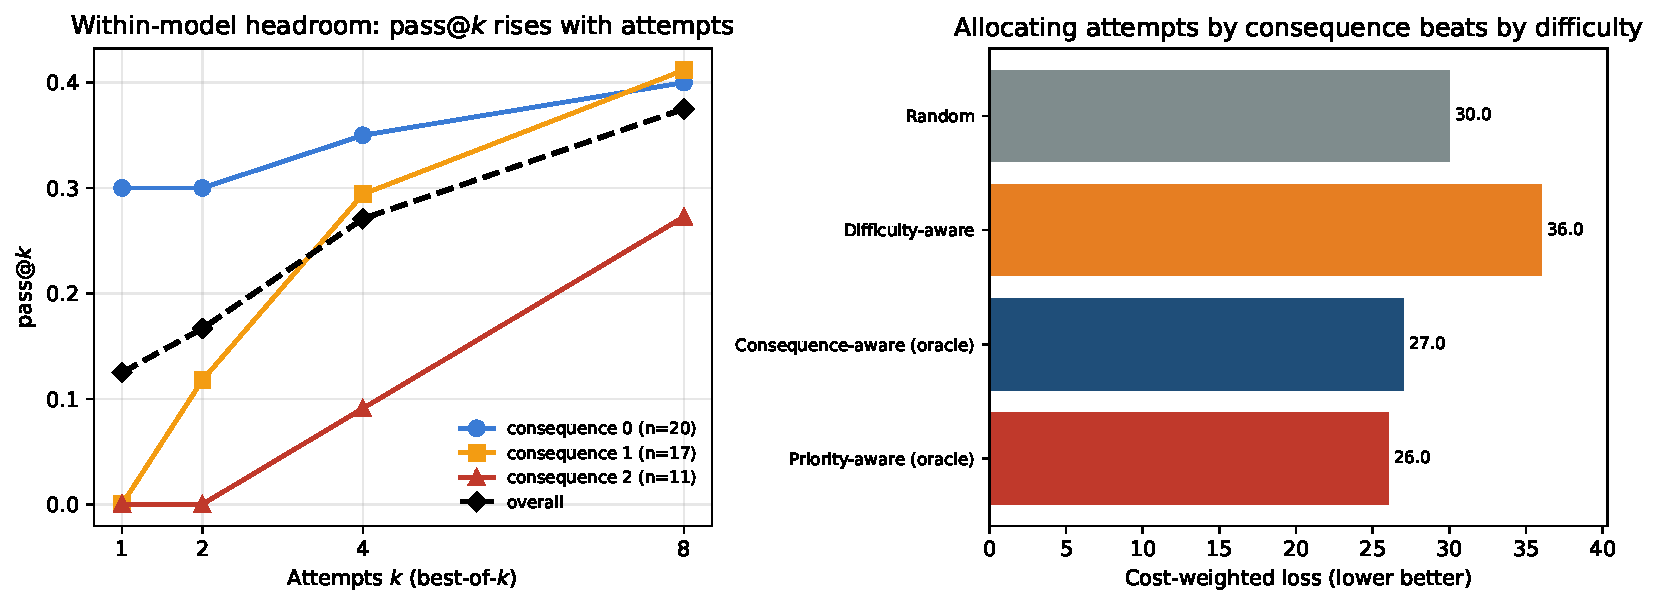
\includegraphics[width=\linewidth]{fig_within.pdf}
\caption{\textbf{Within-model allocation with a single fixed agent.}
\emph{Left:} best-of-$k$ pass rate rises with the number of attempts,
giving real within-model compute headroom (overall
$\mathrm{pass@}1 = 0.125 \to \mathrm{pass@}8 = 0.375$).
\emph{Right:} at a matched total budget of $216$ attempts, allocating attempts by
consequence (or by priority) reduces cost-weighted loss well below the
difficulty-aware baseline, which is itself worse than random ---
reproducing the cross-model main result with the model held fixed.}
\label{fig:within}
\end{figure}

\end{document}